% Force arXiv to process with pdflatex.
\pdfoutput=1

% Support alternating row colours in tables. Normal usage is to
% include the xcolor package with option `table', but the xcolor
% package is already getting pulled in from somewhere else which
% causes builds to fail with a package options conflict.
%
% See: http://tex.stackexchange.com/a/5375
%
\PassOptionsToPackage{table}{xcolor}

\documentclass{article}

\usepackage{arxiv}
\usepackage[utf8]{inputenc} % allow utf-8 input
\usepackage[T1]{fontenc}    % use 8-bit T1 fonts

\rhead{\textsc{ProGraML}: Graph-based Deep Learning for Program Optimization and Analysis}

% Maths.
\usepackage{bm}
\usepackage{amsfonts}
\usepackage{amsmath}

% Tables.
\usepackage{booktabs}
\usepackage{tabularx}
\usepackage{hhline}
\usepackage{xspace}
\usepackage[table]{xcolor}
\usepackage{multirow}
\usepackage{subcaption}
% Define column types L, C, R with known text justification and fixed widths:
\usepackage{array}
\newcolumntype{L}[1]{>{\raggedright\let\newline\\\arraybackslash\hspace{0pt}}m{#1}}
\newcolumntype{C}[1]{>{\centering\let\newline\\\arraybackslash\hspace{0pt}}m{#1}}
\newcolumntype{R}[1]{>{\raggedleft\let\newline\\\arraybackslash\hspace{0pt}}m{#1}}

% \usepackage{subfig}

% Reset footnote counter on every page.
\usepackage{perpage}
\MakePerPage{footnote}

% Add \cmark and \xmark for check and cross symbols, respectively.
\usepackage{amssymb}
\usepackage{pifont}
\newcommand{\cmark}{\ding{51}}%
\newcommand{\xmark}{\ding{55}}%
% Images
\usepackage{graphicx}

\newcommand\todo[2]{\textcolor{red}{\footnotesize \emph{TODO(#1): #2}}}
\newcommand{\bigo}{\mathcal{O}}
\newcommand{\ourproject}{ML4PL}

\usepackage{dsfont}

\title{ProGraML: Graph-based Deep Learning for\\Program Optimization and Analysis}

\author{%
  Chris Cummins\thanks{Both authors contributed equally}\\
  School of Informatics \\
  University of Edinburgh \\
  \texttt{c.cummins@ed.ac.uk} \\
  \And
  Zacharias V. Fisches\textsuperscript{*}\\
  Department of Computer Science \\
  ETH Zurich \\
  \texttt{zfisches@student.ethz.ch} \\
  \And
  Tal Ben-Nun \\
  Department of Computer Science \\
  ETH Zurich \\
  \texttt{talbn@inf.ethz.ch} \\
  \And
  Torsten Hoefler \\
  Department of Computer Science \\
  ETH Zurich \\
  \texttt{htor@inf.ethz.ch} \\
  \And
  Hugh Leather \\
  School of Informatics \\
  University of Edinburgh \\
  \texttt{hleather@inf.ed.ac.uk} \\
}

\begin{document}

\maketitle
\begin{abstract}
Deep learning solves hard compiler problems.
\end{abstract}


\section{Introduction}

This chapter reviews research in areas relevant to this thesis. Section~\ref{sec:related-work-generation} reviews the literature of program generation, focusing on compiler testing and benchmarking. Then Section~\ref{sec:related-work-optimisation} reviews the literature of program optimisation, starting with empirical techniques, iterative compilation, and machine learning. Section~\ref{sec:related-work-other} surveys the literature of relevant works in machine learning for programming languages. Finally Section~\ref{sec:related-work-summary} concludes.

\section{The Case for Benchmark Generators}%
\label{subsec:the-case-for-benchmark-generators}

\begin{figure}[t]
  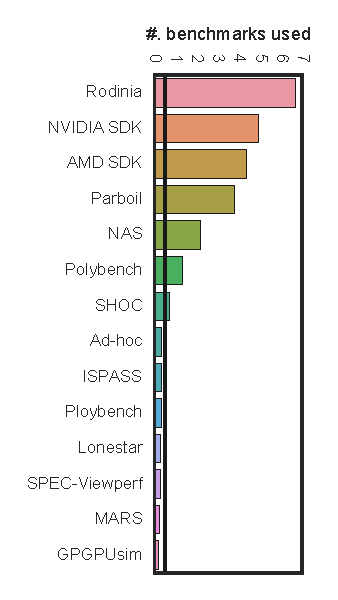
\includegraphics[width=\columnwidth]{img/motivation-c} %
  \caption{%
    The average number of benchmarks used in GPGPU research papers published between 2013-2016 in CGO, HiPC, PACT, and PPoPP.%
  }%
  \label{fig:benchmark-suite-distribution}
\end{figure}

\begin{table}
  \centering%
  \begin{tabular}{ R{1.5cm} C{1.5cm} C{1.5cm} C{1.5cm} C{1.5cm} C{1.5cm} C{1.5cm} C{1.5cm} }
    \toprule
    & \textbf{AMD} & \textbf{NPB} & \textbf{NVIDIA} & \textbf{Parboil} & \textbf{Polybench} & \textbf{Rodinia} & \textbf{SHOC}\\
    \midrule
    \textbf{AMD} & - & 38.0\% & 74.5\% & 76.7\% & 21.7\% & 45.8\% & 35.9\%\\
    \textbf{NPB} & 22.7\% & - & 45.3\% & 36.7\% & 13.4\% & 16.1\% & 23.7\%\\
    \textbf{NVIDIA} & 29.9\% & 37.9\% & - & 21.8\% & 78.3\% & 18.1\% & 63.2\%\\
    \textbf{Parboil} & 89.2\% & 28.2\% & 28.2\% & - & 41.3\% & 73.0\% & 33.8\%\\
    \textbf{Polybench} & 58.6\% & 30.8\% & 45.3\% & 11.5\% & - & 43.9\% & 12.1\%\\
  \textbf{Rodinia} & 39.8\% & 36.4\% & 29.7\% & 36.5\% & 46.1\% & - & 59.9\%\\
  \textbf{SHOC} & 42.9\% & 71.5\% & 74.1\% & 41.4\% & 35.7\% & 81.0\% & -\\
  \end{tabular}
  \caption{Performance relative to the optimal of the \emph{Grewe et al.\ }predictive model across different benchmark suites on an AMD GPU. The columns show the suite used for training; the rows show the suite used for testing.}%
  \label{tab:cpu-gpu-benchmarks-crossvalidate}
\end{table}

In this section we make the argument for synthetic benchmarks. We identified frequently used benchmark suites in a survey of 25 research papers in the field of GPGPU performance tuning from four top tier conferences between 2013--2016: CGO, HiPC, PACT, and PPoPP. We found the average number of benchmarks used in each paper to be 17, and that a small pool of benchmarks suites account for the majority of results, shown in Figure~\ref{fig:benchmark-suite-distribution}. We selected the 7 most frequently used benchmark suites (accounting for 92\% of results), and evaluated the performance of the state of the art \emph{Grewe et   al.}~\cite{Grewe2013} predictive model across each. The model predicts whether running a given OpenCL kernel on the GPU gives better performance than on the CPU. We describe the full experimental methodology in Section~\ref{sec:methodology}.

Table~\ref{cpu-gpu-benchmarks-crossvalidate} summarizes the results. The performance of a model trained on one benchmark suite and used to predict the mapping for another suite is generally very poor. The benchmark suite which provides the best results, NVIDIA SDK, achieves on average only 49\% of the optimal performance. The worst case is when training with Parboil to predict the optimal mappings for Polybench, where the model achieves only 11.5\% of the optimal performance. From this it is clear that heuristics learned on one benchmark suite fail to generalize across other suites.

This problem is caused both by the limited number of benchmarks contained in each suite, and the distribution of benchmarks within the feature space. Figure~\ref{fig:pca-benchmarks} shows the feature space of the Parboil benchmark suite, showing whether, for each benchmark, the model was able to correctly predict the appropriate optimization.  We used Principle Component Analysis to reduce the multi-dimensional feature space to aid visualization.

As we see in Figure~\ref{fig:pca-benchmarks-a}, there is a dense cluster of neighboring benchmarks, a smaller cluster of three benchmarks, and two outliers. The lack of neighboring observations means that the model is unable to learn a good heuristic for the two outliers, which leads to them being incorrectly optimized. In Figure~\ref{fig:pca-benchmarks-b}, we hand-selected benchmarks which are neighbouring in the feature space and retrained the model. The addition of these observations (and the information they provide about that part of the feature space) causes the two outliers to be correctly optimized. We found such outliers in all of the benchmark suites of Table~\ref{tab:benchmark-xval}.

\begin{figure}
  \subfloat[]{%
    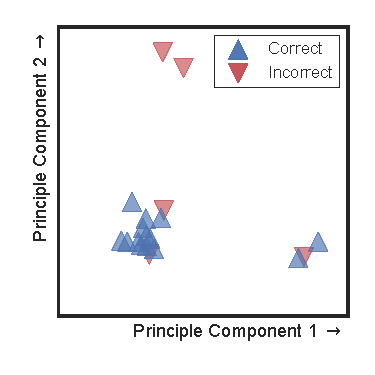
\includegraphics[width=.45\columnwidth]{img/motivation-a}%
    \label{fig:pca-benchmarks-a}%
  }%
  \subfloat[]{%
    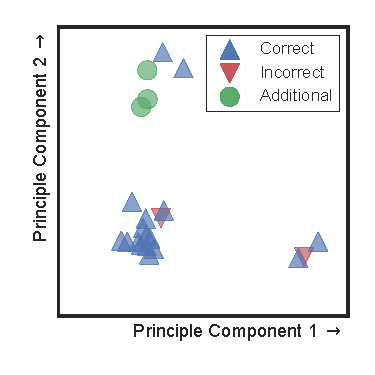
\includegraphics[width=.45\columnwidth]{img/motivation-b}%
    \label{fig:pca-benchmarks-b}%
  }%
  \caption{A two dimensional projection of the \emph{Grewe et al.\ }feature space, showing predictive model results over Parboil benchmarks on an NVIDIA GPU. Two outliers in~\protect\subref{fig:pca-benchmarks-a} are incorrectly predicted due to the lack of nearby observations. The addition of neighboring observations in~\protect\subref{fig:pca-benchmarks-b} corrects this.}%
  \label{fig:pca-benchmarks}
\end{figure}

These results highlight the significant effect that the number and distribution of training programs has on the quality of predictive models. Without good coverage of the feature space, any machine learning methodology is unlikely to produce high quality heuristics, suitable for general use on arbitrary real applications, or even applications from different benchmark suites. Our novel approach, described in the next section, solves this problem by generating an unbounded number of programs to cover the feature space with fine granularity.

\section{A Graphical Program Representation for Analysis and Optimization}
\label{sec:graph-representation}

For machine learning to successfully reason over programs, a suitable
input representation must be used. This section presents
\textsc{ProGraML}, a novel program representation that closely matches
the representations used traditionally within compilers and can be
processed natively by machine learning models. Unlike prior approaches
that rely on hand-engineered feature
extractors~\cite{Ashouri2018,Wang2018} or which are closely tied to
the syntax of the target program language~\cite{Allamanis2017b}, our
approach captures whole-program control, data, and call relations and
is both task- and language-agnostic.

\begin{figure*}
  \centering %
  \begin{subfigure}{.48\linewidth}%
    \centering
    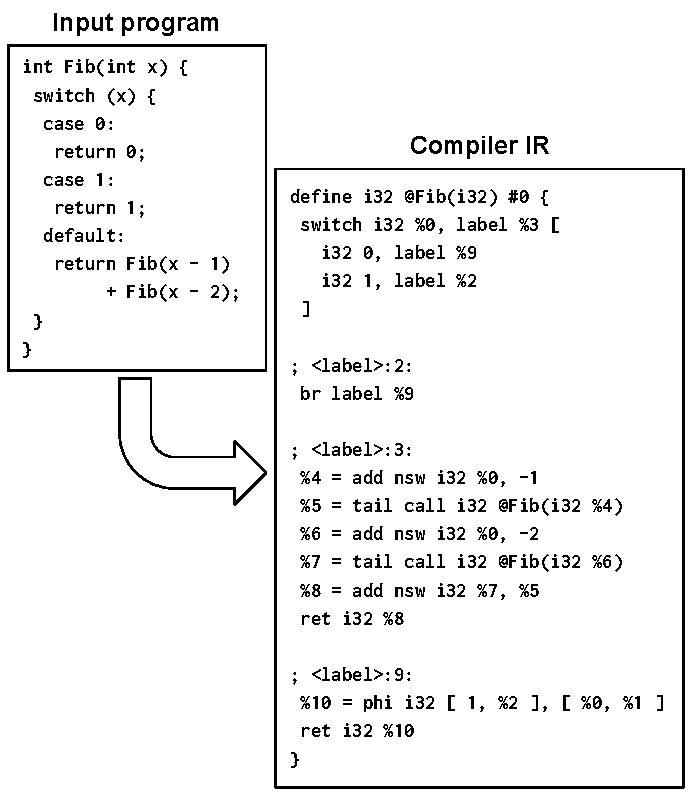
\includegraphics[width=\linewidth]{images/A_IR}%
    \caption{Compiler intermediate representation.}
    \label{subfigure:ir}%
  \end{subfigure}
  \begin{subfigure}{.48\linewidth}%
    \centering
    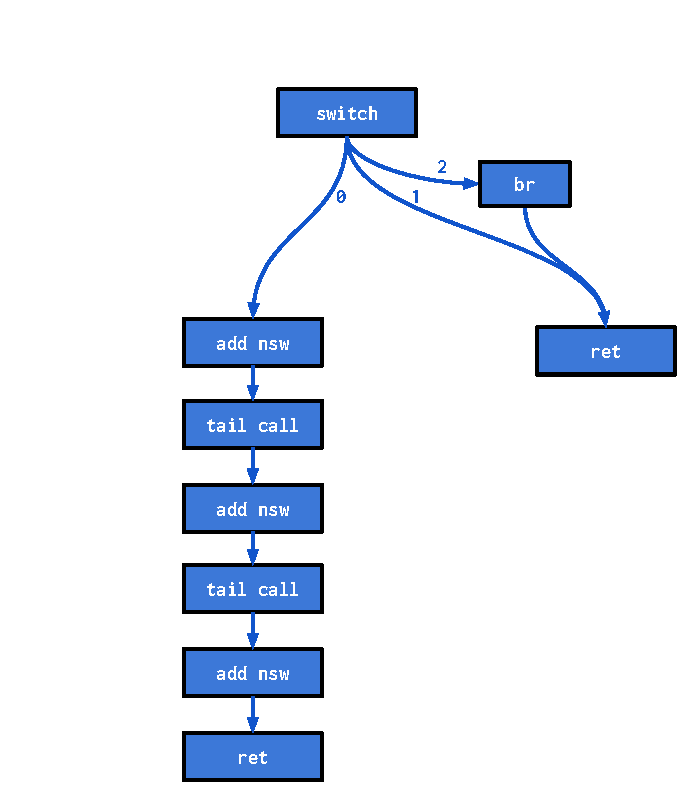
\includegraphics[width=\linewidth]{images/B_Control}%
    \caption{Construct control flow.}
    \label{subfigure:control_flow}%
  \end{subfigure}
  \\*
  \vspace{1em}
  \begin{subfigure}{.48\linewidth}%
    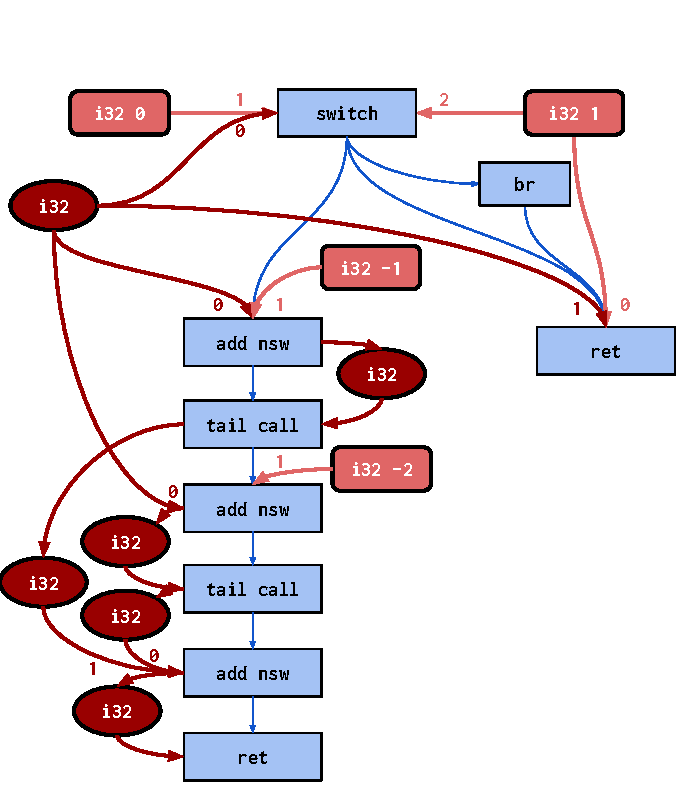
\includegraphics[width=\linewidth]{images/C_Data}%
    \caption{Add data flow for variables and constants.}
    \label{subfigure:data_flow}%
  \end{subfigure}
  \begin{subfigure}{.48\linewidth}%
    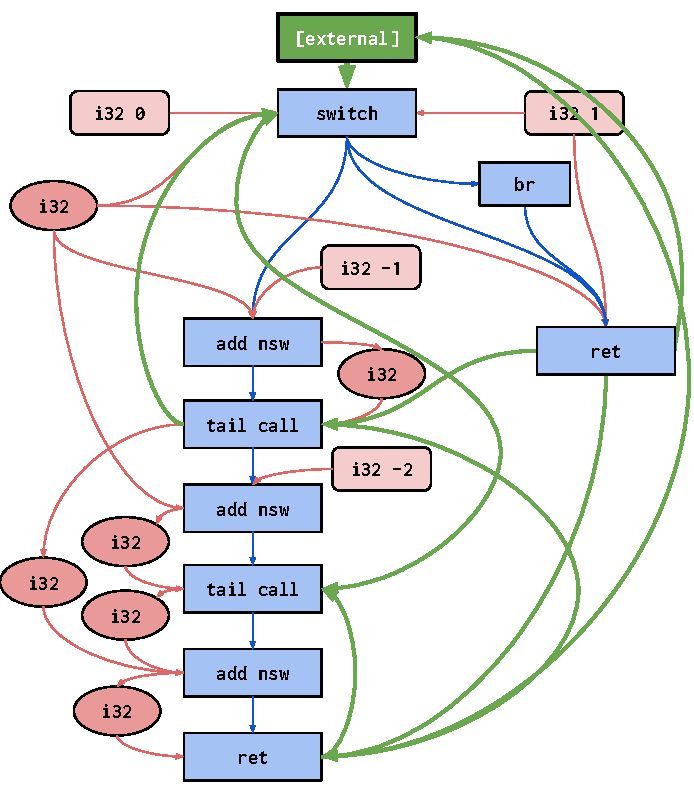
\includegraphics[width=\linewidth]{images/D_Call}%
    \caption{Add call flow for call sites.}
    \label{subfigure:call_flow}%
  \end{subfigure}
  \caption{%
    Construction of a \textsc{ProGraML} representation for a simple C
    implementation of recursive Fibonacci using LLVM-IR. The input
    program is passed through the compiler front end to produce an
    intermediate representation (a). A full flow graph is constructed
    from the IR statements and control flow edges inserted
    (b). Vertices for variables and constant values are  added and
    data-flow edges inserted (c). Finally, call sites are extracted
    and call edges inserted from call sites to function entry
    statements, and from function exit vertices to call sites (d). All
    edges are positional, for clarity we have omitted position labels
    where not required.%
  }%
  \label{figure:graph_construction}%
\end{figure*}

\subsection{Overview}

The \textsc{ProGraML} representation of a compiler IR serves as the
union between a call graph, control-flow graph, and data-flow
graph. We represent programs as directed multigraphs where statements,
identifiers, and immediate values are vertices, and relations between
vertices are edges. Edges are typed to differentiate control-, data-,
and call-flow. Additionally, we augment edges with a positional label
to encode the order of operands for statements, and to differentiate
between divergent branches in control-flow. The \textsc{ProGraML}
representation is processed natively by our machine learning models,
described in Section~\ref{sec:graph-based-machine-learning}.

\subsection{Graph Construction}

We construct a \textsc{ProGraML} graph $G = (V, E)$ by traversing a
compiler IR. Graph construction is divided into three stages:
control-flow, data-flow, and call-flow, though in practice the three
stages can be combined in a single $\bigo{(|V|+|E|)}$ pass. The
representation is compiler-agnostic, adding support for a new compiler
requires only a parser for the IR. Currently we support
LLVM~\cite{Lattner2004} and XLA HLO~\cite{Leary2017}
IRs. Figure~\ref{figure:graph_construction} shows the graph
construction approach.

\paragraph{(I) Control Flow} We construct a full-flow graph from an IR
by inserting a graph vertex for each instruction and control flow
edges between them, as shown in
Figure~\ref{subfigure:control_flow}. All control edges are augmented
with a numeric position label using an ascending sequence based on
their order in the list of a vertex's outgoing control edges. For
instructions with a single control successor, the position of the
control edge is 0. For a branching statement with $n$ successor
statements, the control edge positions are in the range
$0 \le e_{\text{pos}} \le n$. We do not need to encode the source
function or basic block~\cite{Lattner2004} of instructions as this
information is captured implicitly in structure of the graph; basic
blocks are regions of instructions with a single entry and exit
control edge, and functions are disconnected subgraphs.

\paragraph{(II) Data Flow} We introduce additional graph vertices for
constant values and variables, shown in
Figure~\ref{subfigure:data_flow}. Data-flow edges are added to capture
the relation from constants and variables to the instructions that use
them as operands, and instructions to produced variables. Each unique
variable and constant is a vertex, which implicitly models the scope
of variables, and unlike the tokenized representations of prior
machine learning works, variables in different scopes always map to
distinct vertices and can thus be discerned. Similarly, constant
values with the same textual representation in source code (such as
the number \texttt{3.14} with \texttt{float} and \texttt{double}
precision types) are distinguishable in our representation. As with
control edges, data edges have a position label which encodes the
order of operands for instructions. The latent representation of an IR
statement is thus a function of the vertex representing the
instruction and the vertices of any operand variables or constants,
modulated by their order in the list of operands.

\paragraph{(III) Call Flow} Control edges do not span functions, such
that an IR with functions $F$ produces $|F|$ disconnected subgraphs
(the same is not true for data edges which may cross function
boundaries, for example in the case of an global constant which is
used within multiple functions of a program). Instead, the relation
between a statement which calls a function and the called function is
captured through call edges, shown in
Figure~\ref{subfigure:call_flow}. An outgoing call edge is inserted
from the calling statement to the entry statement of a
function. Return call edges are added from all terminal statements of
a function to the calling statement. Call edges do not use position
labels as there is no ordering to be imposed between the call sites of
a function. For IRs which support external linkage, an additional
vertex is created representing an external callsite and connected to
all externally visible functions. Similarly, if a call site references
a function not defined in the current IR, a \emph{dummy} function
definition is created consisting of a pair of entry and exit
instruction vertices, and connected normally through call edges. A
single dummy function definition is created for each externally
defined function and shared across all call sites in the current IR.


\subsection{Comparison to Other Representations}

As an input for machine learning, what distinguishes \textsc{ProGraML}
from prior works is its close proximity to the structured
representations traditionally used within compilers for program
analysis and optimization. Specifically, it is distinct from prior
machine learning representations in three key areas:
\begin{enumerate}
\item as an IR-level representation, it is independent of the source
  language and accompanying variances such as code style and
  identifier naming that affect source-level
  representations~\cite{Alon2018a,Cummins2017a};
\item by representing programs as graphs with explicit control, data,
  and call edge types \textsc{ProGraML} captures a greater range of
  intra-program relations than prior graph
  representations~\cite{Ben-nun2018,Allamanis2017b,Park2012};
\item and in trading sequential for graph representations, we do not
  sacrifice local sequence order, such as the ordering of diverging
  control flow or the ordering of operands that is lost in prior
  representations~\cite{Ben-nun2018,Brauckmann2020}.
\end{enumerate}

Table~\ref{tab:representation_taxonomy} provides a comparison of
\textsc{ProGraML} to several recent learned representations of code.

\begin{table}
  \centering
  \footnotesize
  \begin{tabular}{r L{3.6cm} L{2.5cm} L{1.8cm} L{1.8cm} L{1.8cm}}
    \toprule
    & Source Languages & Representation & Flow-sensitive? & Position-sensitive? & Value-sensitive? \\
    \midrule
    AST Paths~\cite{Alon2018c} & C\#, Java, JavaScript, Python & AST & &  & \cmark \\
    CDFG~\cite{Brauckmann2020} & OpenCL & IR Graph & \cmark &  &  \\
    code2vec~\cite{Alon2018a} & Java & AST & & & \cmark \\
    DeepTune~\cite{Cummins2017b} & OpenCL & Token Sequence &  & \cmark & \cmark \\
    DeepTune-IR\cite{Barchi2019a} & OpenCL & IR Token Sequence &  & \cmark & \\
    DeepTyper~\cite{Hellendoorn2018} & JavaScript & Token Sequence &  & \cmark & \cmark \\
    inst2vec~\cite{Ben-nun2018} & C++, OpenCL & IR Graph & \cmark & & \cmark \\
    \textbf{\textsc{ProGraML}} & \textbf{C, C++, Fortran, Haskell, OpenCL, Swift} & \textbf{IR Graph} & \cmark & \cmark & \cmark \\
    \bottomrule
  \end{tabular}
  \vspace{.3em}
  \caption{%
    Taxonomy of recent code representations for machine learning. We
    classify approaches based on the type of representation used and
    the sensitivity to three categories: \{control/data/call\}-flow,
    operand positions, and operand values. Prior approaches require a
    trade-off in representational power, e.g. substituting a
    position-sensitive token sequence for a flow-sensitive
    graph. \textsc{ProGraML} is the first representation to span all
    categories.%
  }%
  \label{tab:representation_taxonomy}
\end{table}

\section{Graph-based Machine Learning}
\label{sec:graph-based-machine-learning}

We formulate our system in a Message Passing Neural Network (MPNN)
framework~\cite{Gilmer2017,Li2015a} and implement a single unified
model for all our experiments. Our design mimics the \emph{transfer
  functions} and \emph{meet operators} of classical iterative dataflow
analysis~\cite{Kam1977,Cooper2003}, replacing the rule-based
implementations with deep learning analogues (message and update
functions). Those can be specialized through training to solve a
diverse set of problems without human intervention or algorithm
design.


\subsection{Overview}

We learn over \textsc{ProGraML} representations of compiler IRs by
mapping graph vertices to an initial state vector using an
embedding. The vertex states are updated iteratively in a sequence of
message passing steps, where at each step a new vertex state is
computed as a function of its previous state and the state of its
neighboring vertices. Separate functions are learned to update vertex
neighbors based on their relation type, be it control, data or call,
and reverse edges enable backwards propagation of information. After
repeating this process of updating vertex states for a fixed number of
iterations a readout function is used to aggregate the vertex
representations to a single graph-level vector or set of vertex-level
vectors.


\subsection{Model Design}

The \textsc{ProGraML} model takes as input a directed graph with
additional information as presented in
Section~\ref{sec:graph-representation} and consists of three logical
phases: input encoding, message propagation, and result readout.

\paragraph{(I) Input Encoding} Starting from the augmented graph
representation $G = (V, E)$ introduced in Section
\ref{sec:graph-representation}, we capture the semantics of the
program graph vertices by mapping every instruction, constant, and
variable vertex $v \in V$ to a vector representation
$h_v^0 \in \mathbb{R}^{d}$ by lookup in a fixed size embedding table
$C_ \text{IR} \in \mathbb{R}^{n \times d}$. The mapping from vertex to
embedding vector $f: v \hookrightarrow h_v^0 \in C_\text{IR}$ must be
defined for each IR, though the embeddings themselves can be learned
during training.

For LLVM-IR we extend the inst2vec~\cite{Ben-nun2018} vocabulary,
which represents 8,566 statements derived from a large corpus of
LLVM-IR using 200-dimensional embeddings. Since the space of
statements is unbounded, inst2vec uses a normalization process to
inline type definitions and strip identifiers and immediate values,
depicted in Figure~\ref{fig:embedding}. An inst2vec representation
combines an instruction and its operands into a single token, so we
augment the vocabulary with \textsc{Id} and \textsc{Val} tokens to
represent variable and constant value vertices, respectively.

In expressing a statement as a combination of an instruction and its
operands, our data-driven approach trades a certain amount of semantic
resolution against good coverage of the vocabulary by the available
datasets. The long tail of the distribution of statements jointly maps
onto a special \textsc{Unknown} token vector in the vocabulary. In
future work will simplify the LLVM-IR statement encoding by
constructing separate vocabularies for instructions and operand types,
increasing the expressiveness of the encoding by allowing a larger
combination of instruction and operands to be represented.  Input
\emph{vertex-selectors}, encoded as binary one-hot vectors, are used
to mark the starting point for certain analyses and are concatenated
to the vertex
embeddings.
Other global input features are used as auxiliary input features at
readout time in step (III), where required.

\begin{figure}
  \centering
  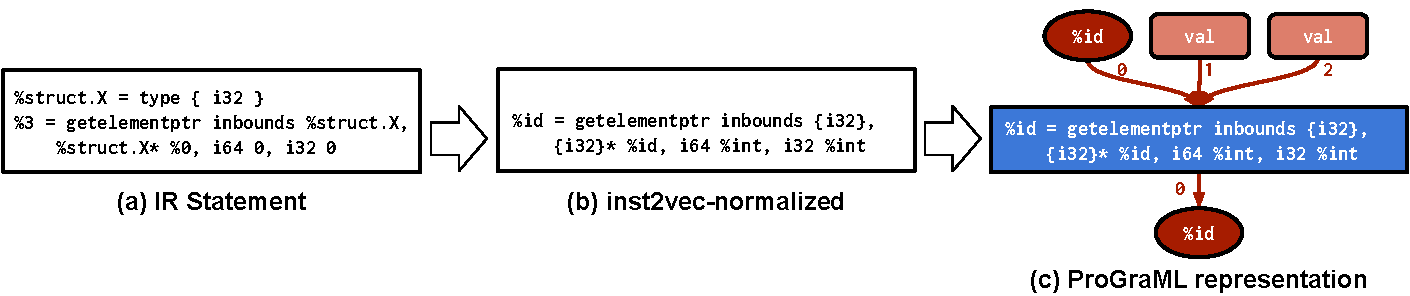
\includegraphics[width=\linewidth]{images/embedding}%
  \caption{%
    Normalizing an LLVM-IR statement (a) by inlining type definitions
    and stripping identifiers using inst2vec~\cite{Ben-nun2018} (b). A
    normalized statement is used as the key for an embedding table
    lookups to produce the initial vector representation of a
    vertex. (c) shows the statement as contextualized in a
    \textsc{ProGraML} graph, where the operand variables and constants
    are data elements, differentiated by their position. Vertex labels
    represent embedding table keys. In this example, the statement is
    represented using five vertices and encoded with three unique
    embeddings.%
  }%
  \label{fig:embedding}%
\end{figure}

\paragraph{(II) Message Propagation} Each iteration step is divided
into a message propagation step followed by a vertex state
update. During message propagation, each vertex in the graph collects
learned messages $m_v^{t} \in \mathbb{R}^d$ from its undirected
neighbors:

\begin{equation}
  m^t_{v} = \sum_{w \in \mathcal{N}(v)} A_{\mathrm{type}(e_{wv})}\,  (h_w^{t-1} \odot \textsc{pos}(e_{wv}))\,
\end{equation}

where $\odot$ denotes the Hadamard product and $e_{wv} \in E$ is the
typed edge between vertex $w$ and $v$. In order to allow for
reverse-propagation of messages, which is necessary for backward
compiler analyses, we add backward edges for each edge in the
graph. For backward edges we introduce separate parameters following
Li et al.~\cite{Li2015a} to enable the network to distinguish between
an edge and its backward sibling. During message propagation we scale
the source states $h_v^{t-1}$ with
\textsc{pos}$(\cdot) \in \mathbb{R}^d$, which is a constant sinusoidal
position embedding~\cite{Vaswani2017,Gehring2017} that encodes the
argument order of incoming (and outgoing) edges. This information is
necessary for the network to distinguish non-commutative operations
such as division.

The collected messages are subsequently used to update the vertex
states $h_{v} \in \mathbb{R}^d$ in parallel according to an update
function. In all our experiments, we employ a Gated Recurrent Unit
(GRU) \cite{Cho2014} as our update function:

\begin{equation}
h_v^t = \textsc{Gru}(h_v^{t-1}, m_v^t)
\end{equation}

Step (II) is iterated $T$ times to extract vertex representations that
are contextualized with respect to the given graph structure.

\paragraph{(III) Result Readout} We support whole program
classification, per-statement classification, or per-identifier
classification by employing different \emph{readout heads} on top of
the iterated feature extraction: for graph-level classification we
define a set function $R_G(\{h_v^T, h_v^0\}_{v \in V})$ that maps to
class-scores, while for vertex-level inference, we separately map the
extracted node features $h_v^T$ to probabilities $R_v(h_v^T, h_v^0)$
in parallel:
\begin{align}
  R_{v}(h_v^T, h_v^0) &= \sigma\left(i(h_v^T, h_v^0)\right) \cdot j(h_v^T) \\
  R_{G}(\{h_v^T, h_v^0\}_{v \in V}) &= \sum\limits_{v \in V}\,\,R_{v}(h_v^T, h_v^0)
\end{align}
where $i(\cdot)$ and $j(\cdot)$ are feed forward Neural Networks and
$\sigma(\cdot)$ is the sigmoid activation function.  In the case where
auxiliary graph-level features are available, those are concatenated
to the readout values and fed through another feed forward Neural
Network that employs Batch Normalization~\cite{Ioffe2015a} to allow
for vastly different feature scales.

\section{Case Study A: OpenCL Heterogeneous Mapping}
\label{sec:deeptune-case-study-a}

OpenCL provides a platform-agnostic framework for heterogeneous parallelism. This allows a program written in OpenCL to execute transparently across a range of different devices, from CPUs to GPUs and FPGAs. Given a program and a choice of execution devices, the question then is on which device should one execute the program to maximise performance?

\subsection{State-of-the-art}

We return to the \emph{Grewe et al.\ }~\cite{Grewe2013} predictive model of Chapter~\ref{chap:clgen} for mapping OpenCL kernels to the optimal device in CPU/GPU heterogeneous systems. They use supervised learning to construct decision trees, using a combination of static and dynamic kernel features. The static program features are extracted using a custom LLVM pass; the dynamic features are taken from the OpenCL runtime.

\paragraph*{Expert Chosen Features}

Table~\ref{tab:grewe-features-final} shows the features used in their work. Each feature is an expression built upon the code and runtime metrics given in Table~\ref{tab:grewe-features-raw}.

\begin{table}
  \rowcolors{2}{gray!25}{white}
  \centering%
  \subfloat[Feature values]{
    \begin{tabular}{| l L{4.5cm} |}
      \hline
      \rowcolor{gray!50}
      \textbf{Name} & \textbf{Description} \\
      \hline
      \texttt{F1: data size/(comp+mem)} & commun.-computation ratio \\
      \texttt{F2: coalesced/mem} & \% coalesced memory accesses \\
      \texttt{F3: (localmem/mem)$\times$wgsize} & ratio local to global mem accesses  $\times$ \#.\ work-items \\
      \texttt{F4: comp/mem} & computation-mem ratio\\
      \hline
    \end{tabular}%
    \label{tab:grewe-features-final}%
  }\\ %
  \subfloat[Values used in feature computation]{%
    \rowcolors{2}{gray!25}{white}
    \begin{tabular}{| l c l |}
    	\hline
      \rowcolor{gray!50}
      \textbf{Name} & \textbf{Type} & \textbf{Description} \\
      \hline
      \texttt{comp} & static & \#.\ compute operations \\
      \texttt{mem} & static & \#.\ accesses to global memory \\
      \texttt{localmem} & static & \#.\ accesses to local memory \\
      \texttt{coalesced} & static & \#.\ coalesced memory accesses \\
      \texttt{data size} & dynamic & size of data transfers \\
      \texttt{work-group size} & dynamic & \#.\ work-items per kernel \\
      \hline
    \end{tabular}%
    \label{tab:grewe-features-raw}%
  }
  \caption[Heterogeneous mapping model features]{%
    Features used by \emph{Grewe et al. }to predict heterogeneous device
    mappings for OpenCL kernels.%
  } %
  \label{tab:grewe-features} %
\end{table}


\subsection{Experimental Setup}

The predictive model of \emph{Grewe et al.\ }~\cite{Grewe2013} is replicated. The same experimental setup is used as in Chapter~\ref{chap:clgen} in which the experiments are extended to a larger set of 71 programs, summarised in Table~\ref{tab:cgo-benchmarks}. The programs were evaluated on two CPU-GPU platforms, detailed in Table~\ref{tab:cgo-platforms}.

\begin{table}
	\centering%
	\rowcolors{2}{gray!25}{white}
	\begin{tabular}{| l r r r |}
		\hline
		\rowcolor{gray!50}
		& \textbf{Version} & \textbf{\#. benchmarks} & \textbf{\#. kernels}\\
		\hline
		\textbf{NPB (SNU~\cite{Seo2011})} & 1.0.3 & 7 & 114 \\
		\textbf{Rodinia~\cite{Che2009}} & 3.1 & 14 & 31 \\
		\textbf{NVIDIA SDK} & 4.2 & 6 & 12 \\
		\textbf{AMD SDK} & 3.0 & 12 & 16 \\
		\textbf{Parboil~\cite{Stratton2012}} & 0.2 & 6 & 8 \\
		\textbf{PolyBench~\cite{Grauer-Gray2012}} & 1.0 & 14 & 27 \\
		\textbf{SHOC~\cite{Danalis2010}} & 1.1.5 & 12 & 48 \\
		\textbf{Total} & - & 71 & 256 \\
		\hline
	\end{tabular}
  \caption[Benchmarks used in Case Study A]{%
	  Benchmarks used in Case Study A.%
  }
	\label{tab:cgo-benchmarks}
\end{table}

\begin{table}[t!]
	\centering %
		\rowcolors{2}{gray!25}{white}
		\begin{tabular}{| l l l l| }
			\hline
			\rowcolor{gray!50}
			& \textbf{Frequency} & \textbf{Memory} & \textbf{Driver} \\
			\hline
			\textbf{Intel Core i7-3820} & 3.6 GHz & 8GB & AMD 1526.3 \\
			\textbf{AMD Tahiti 7970} & 1000 MHz & 3GB & AMD 1526.3 \\
			\textbf{NVIDIA GTX 970} & 1050 MHz & 4GB & NVIDIA 361.42 \\
			\hline
		\end{tabular}
	  \caption[Benchmarks used in Case Study A]{%
		Experimental platforms used in Case Study A.%
  	}
		\label{tab:cgo-platforms}
\end{table}


\paragraph*{DeepTune Configuration} 

Figure~\ref{fig:nn}a shows the neural network configuration of DeepTune for the task of predicting optimal device mapping. The OpenCL kernel source code is used as input, along with the two dynamic values \emph{work-group size} and \emph{data size} available to the OpenCL runtime.

\paragraph*{Model Evaluation} 

\emph{Stratified 10-fold cross-validation} is used to evaluate the quality of the predictive models~\cite{Han2011}. Each program is randomly allocated into one of 10 equally-sized sets; the sets are balanced to maintain a distribution of instances from each class consistent with the full set. A model is trained on the programs from all but one of the sets, then tested on the programs of the unseen set. This process is repeated for each of the 10 sets, to construct a complete prediction over the whole data set.

\begin{figure}[t!]
  \centering
  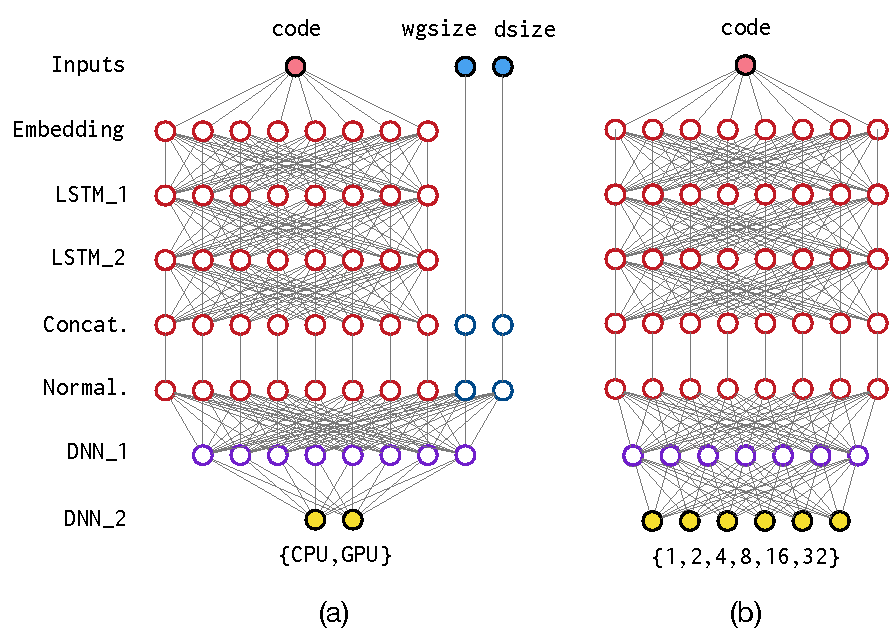
\includegraphics[width=\columnwidth]{img/nn} %
  \caption[DeepTune artificial neural networks]{%
    DeepTune artificial neural networks, configured for (a) heterogeneous mapping, and (b) thread coarsening factor. The design stays almost the same regardless of the optimisation problem. The only changes are the extra input for (a) and size of the output layers.%
  }%
  \label{fig:nn}
\end{figure}



\subsection{Experimental Results}

Selecting the optimal execution device for OpenCL kernels is essential for maximising performance. For a CPU/GPU heterogeneous system, this presents a binary choice. In this experiment, the approach is compared against a static single-device approach and the \emph{Grewe et al.\ }predictive model. The \emph{static mapping} selects the device which gave the best average case performance over all the programs. On the AMD platform, the best-performing device is the CPU; on the NVIDIA platform, it is the GPU.

Figure~\ref{fig:cgo-accuracy} shows the accuracy of both predictive models and the static mapping approach for each of the benchmark suites. The static approach is accurate for only 58.8\% of cases on AMD and 56.9\% on NVIDIA. This suggests the need for choosing the execution device on a per program basis. The \emph{Grewe et al.\ }model achieves an average accuracy of 73\%, a significant improvement over the static mapping. By automatically extracting useful feature representations from the source code, DeepTune gives an average accuracy of 82\%, an improvement over both schemes.

\begin{figure}
	\centering %
	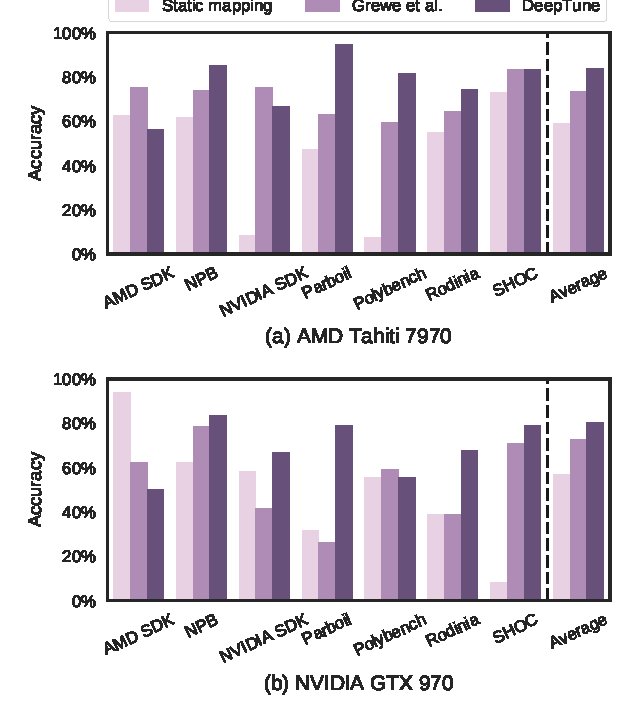
\includegraphics[width=.85\columnwidth]{img/cgo-acc}%
	\caption[Accuracy of optimisation heuristics for heterogeneous device mapping]{%
		Accuracy of optimisation heuristics for heterogeneous device mapping, aggregated by benchmark suite. The optimal static mapping achieves 58\% accuracy. The \emph{Grewe et al. }and DeepTune predictive models achieve accuracies of 73\% and 84\%, respectively.%
	}
	\label{fig:cgo-accuracy}
\end{figure}

Using the static mapping as a baseline, the relative performance of each program is computed using the device selected by the \emph{Grewe et al.\ }and DeepTune models. Figure~\ref{fig:cgo-speedup} shows these speedups. Both predictive models significantly outperform the static mapping; the Grewe \emph{et al.\ }model achieves an average speedup of $2.91\times$ on AMD and $1.26\times$ on NVIDIA (geometric mean $1.18\times$). In 90\% of cases, DeepTune matches or outperforms the predictions of the Grewe \emph{et al.\ }model, achieving an average speedup of $3.34\times$ on AMD and $1.41\times$ on NVIDIA (geometric mean $1.31\times$). This 14\% improvement in performance comes at a greatly reduced cost, requiring no intervention by humans.

\begin{figure}
	\centering %
	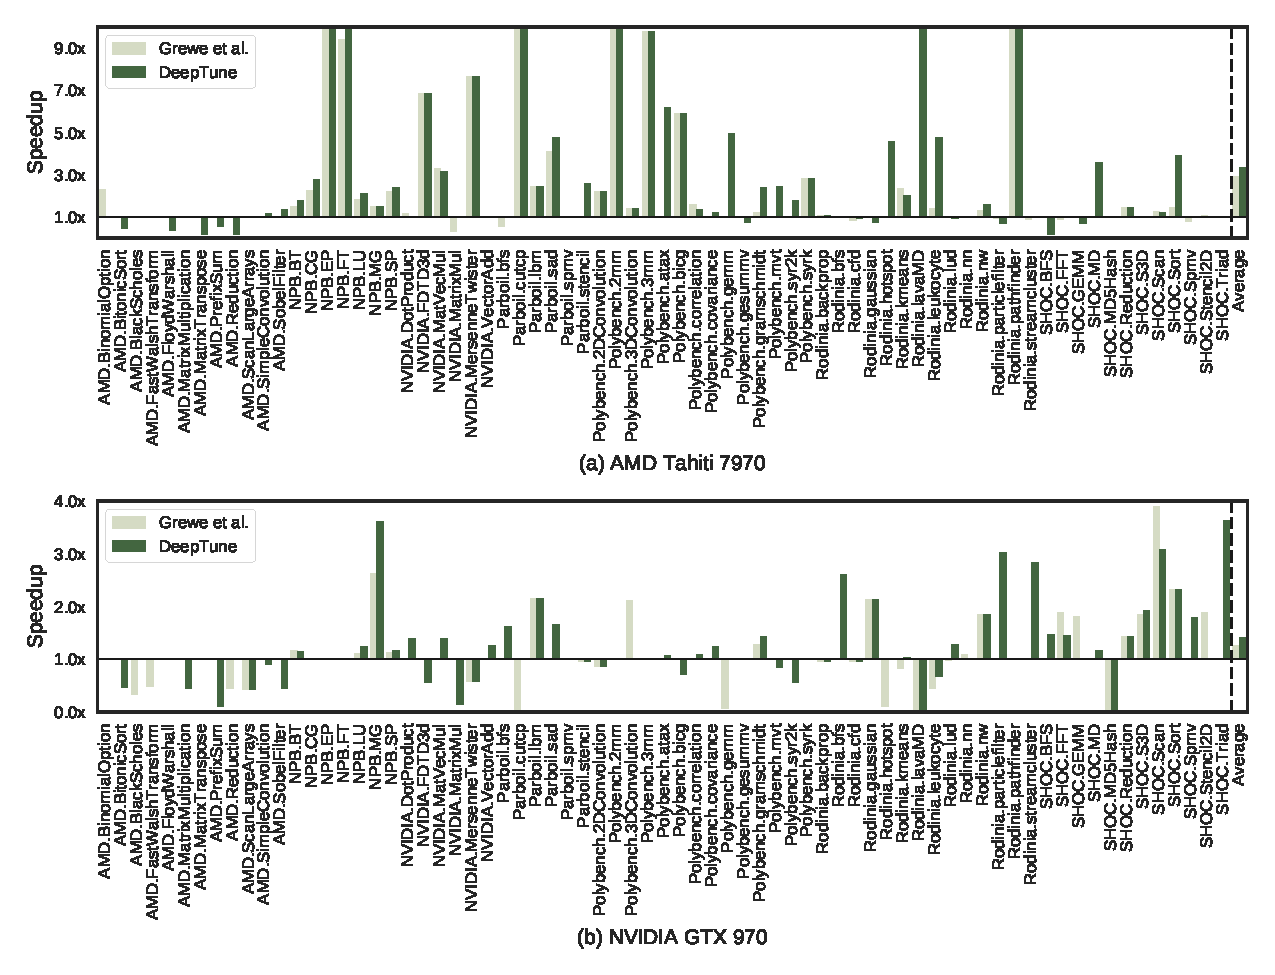
\includegraphics[width=\textwidth]{img/cgo-speedup}%
	\caption[Speedup of predicted heterogeneous mappings]{%
		Speedup of predicted heterogeneous mappings over the best static mapping for both platforms. In (a) DeepTune achieves an average speedup of 3.43x over static mapping and 18\% over \emph{Grewe et al}. In (b) the speedup is 1.42x and 13\% respectively.%
	}
	\label{fig:cgo-speedup}
\end{figure}



\section{Case Study B: OpenCL Thread Coarsening Factor}

Thread coarsening is an optimisation for parallel programs in which the operations of two or more threads are fused together. This optimisation can prove beneficial on certain combinations of programs and architectures, for example programs with a large potential for Instruction Level Parallelism on Very Long Instruction Word architectures.

\subsection{State-of-the-art} \emph{Magni et al.\ }present a predictive model for OpenCL thread coarsening in~\cite{Magni2014}. They implement an iterative heuristic which determines whether a given program would benefit from coarsening. If yes, then the program is coarsened, and the process repeats, allowing further coarsening. In this manner, the problem is reduced from a multi-label classification problem into a series of binary decisions, shown in Figure~\ref{fig:cf-magni}. They select from one of six possible coarsening factors: $(1, 2, 4, 8, 16, 32)$, divided into 5 binary choices.

\begin{figure}
  \centering %
  \subfloat[Magni \emph{et al.\ }cascading binary model.]{%
    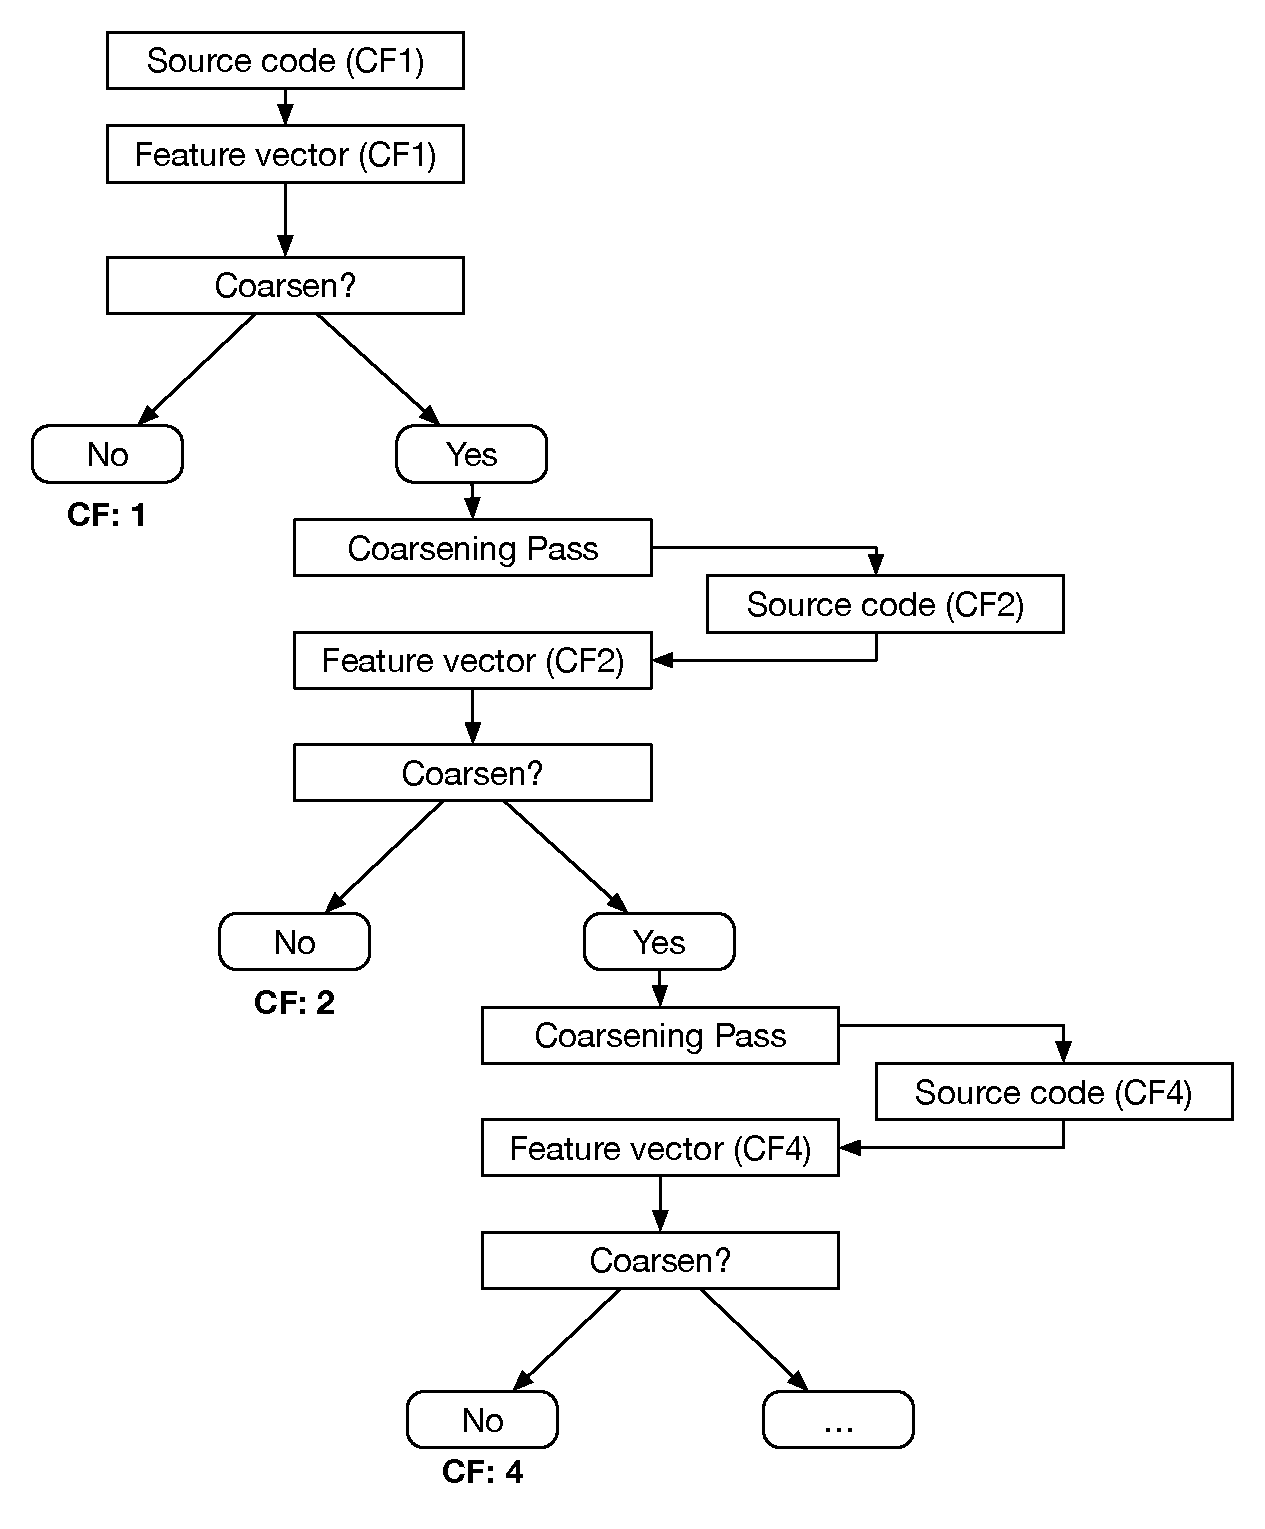
\includegraphics[width=.85\columnwidth]{img/cf-magni}%
    \label{fig:cf-magni}
  }\\*%
  \subfloat[Our approach.]{%
      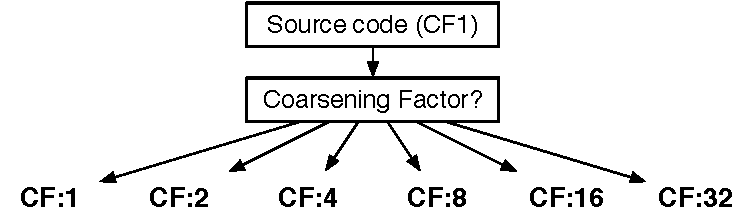
\includegraphics[width=.65\columnwidth]{img/cf-deeptune}%
      \label{fig:cf-deeptune}
  }%
  \caption{%
      Two approaches for predicting coarsening factor (CF) of OpenCL kernels.
      Magni \emph{et al.\ }reduce the multi-label classification problem to a
      series of binary decisions, by iteratively applying the optimization and
      computing new feature vectors. Our approach simply predicts the coarsening
      factor directly from the source code.%
  }
  \label{fig:cascading-nn}
\end{figure}


\begin{table}
  \rowcolors{2}{gray!25}{white}
  \centering%
    \begin{tabular}{| l l |}
      \hline
      \rowcolor{gray!50}
      \textbf{Name} & \textbf{Description} \\
      \hline
      \texttt{BasicBlocks} & \#.\ basic blocks \\
      \texttt{Branches} & \#.\ branches \\
      \texttt{DivInsts} & \#.\ divergent instructions \\
      \texttt{DivRegionInsts} & \#.\ instructions in divergent regions \\
      \texttt{DivRegionInstsRatio} & \#.\ instr. in divergent regions / total instructions \\
      \texttt{DivRegions} & \#.\ divergent regions \\
      \texttt{TotInsts} & \#.\ instructions \\
      \texttt{FPInsts} & \#.\ floating point instructions \\
      \texttt{ILP} & average ILP / basic block \\
      \texttt{Int/FP Inst Ratio} & \#.\ branches \\
      \texttt{IntInsts} & \#.\ integer instructions \\
      \texttt{MathFunctions} & \#.\ match builtin functions \\
      \texttt{MLP} & average MLP / basic block \\
      \texttt{Loads} & \#.\ loads \\
      \texttt{Stores} & \#.\ stores \\
      \texttt{UniformLoads} & \#.\ loads unaffected by coarsening direction \\
      \texttt{Barriers} & \#.\ barriers \\
      \hline
    \end{tabular}%
    \label{tab:features-pact14-raw}%
  \caption[\emph{Magni et al.\ }features for predicting thread coarsening]{%
    Candidate features used by \emph{Magni et al.\ }for predicting thread
    coarsening. From these values, they compute relative deltas for each
    iteration of coarsening, then use PCA for selection.%
  }%
  \label{tab:magni-features} %
\end{table}


\paragraph*{Expert Chosen Features}

\emph{Magni et al.\ }followed a very comprehensive feature engineering process. 17 candidate features were assembled from previous studies of performance counters and computed theoretical values~\cite{Magni2,Sim2012}. For each candidate feature they compute its coarsening \emph{delta}, reflecting the change in each feature value caused by coarsening: $f_{\Delta} = (f_{after} - f_{before}) / f_{before}$, adding it to the feature set. Then they use Principle Component Analysis (PCA) on the 34 candidates and selected the first 7 principle components, accounting for 95\% of variance in the space.

\subsection{Experimental Setup}

The experimental setup of \emph{Magni et al.}~\cite{Magni2014} is replicated. The thread coarsening optimisation is evaluated on 17 programs, listed in Table~\ref{tab:pact-benchmarks}. Four different GPU architectures are used, listed in Table~\ref{tab:pact-platforms}.

\begin{table}
	\centering%
	\rowcolors{2}{gray!25}{white}
	\begin{tabular}{| l r r r |}
		\hline
		\rowcolor{gray!50}
		& \textbf{Version} & \textbf{\#. benchmarks} & \textbf{\#. kernels}\\
		\hline
		\textbf{NVIDIA SDK} & 4.2 & 3 & 3 \\
		\textbf{AMD SDK} & 3.0 & 10 & 10 \\
		\textbf{Parboil~\cite{Stratton2012}} & 0.2 & 4 & 4 \\
		\textbf{Total} & - & 17 & 17 \\
		\hline
	\end{tabular}
	\label{tab:pact-benchmarks}
  \caption[Benchmarks used in Case Study B]{%
	  Benchmarks used in Case Study B.%
  }
\end{table}

\begin{table}[t!]
	\centering %
		\rowcolors{2}{gray!25}{white}
		\begin{tabular}{| l l l l |}
			\hline
			\rowcolor{gray!50}
			& \textbf{Frequency} & \textbf{Memory} & \textbf{Driver} \\
			\hline
			\textbf{AMD HD 5900} & 725 MHz & 2GB & AMD 1124.2 \\
			\textbf{AMD Tahiti 7970} & 1000 MHz & 3GB & AMD 1084.4 \\
			\textbf{NVIDIA GTX 480} & 700 MHz & 1536 MB & NVIDIA 304.54 \\
			\textbf{NVIDIA K20c} & 706 MHz & 5GB & NVIDIA 331.20 \\
			\hline
		\end{tabular}
	  \caption[Experimental platforms used in Case Study B]{%
		Experimental platforms used in Case Study B.%
	}
		\label{tab:pact-platforms}
\end{table}


\paragraph*{DeepTune Configuration}

Figure~\ref{fig:nn}b shows the neural network configuration. The OpenCL kernel is the sole input the coarsening factor is the predicted output.

\paragraph*{Model Evaluation}

Compared to Case Study A, the size of the evaluation is small. We use \emph{leave-one-out cross-validation} to evaluate the models. For each program, a model is trained on data from all other programs and used to predict the coarsening factor of the excluded program.

The parameters of the neural network is not described in~\cite{Magni2014}, so an additional, \emph{nested} cross-validation process is used to find the optimal model parameters. For every program in the training set, 48 combinations of network parameters are evaluated. The best performing configuration is selected from these 768 results to train a model for prediction on the excluded program. This nested cross-validation is repeated for each of the training sets. No such tuning of hyper-parameters is performed for DeepTune.


\subsection{Comparison to Case Study A}

For the two different optimisation heuristics, the authors arrived at very different predictive model designs, with very different features. By contrast, the DeepSmith approach is exactly the same for both problems. None of DeepTune's parameters were tuned for the case studies presented above. Their settings represent conservative choices expected to work reasonably well for most scenarios.

Table~\ref{tab:nn-size} shows the similarity of the models. The only difference between the network designs is the auxiliary inputs for Case Study A and the different number of optimisation decisions. The differences between DeepTune configurations is only two lines of code: the first, adding the two auxiliary inputs; the second, increasing the size of the output layer for Case Study B from two neurons to six. The description of these differences is larger than the differences themselves.

\begin{table}
  \centering
  \rowcolors{2}{white}{gray!25}
  \begin{tabular}{| l r r | r r |}
    \hline
    \rowcolor{gray!50}
    & \multicolumn{2}{c}{\textbf{\#.\ neurons}} & \multicolumn{2}{c}{\textbf{\#.\ parameters}} \\
    \rowcolor{gray!50}
    & \textbf{HM} & \textbf{CF} & \textbf{HM} & \textbf{CF} \\
    \hline
    \textbf{Embedding} & 64 & 64 & ,256 & 8,256 \\
    \textbf{LSTM\_1} & 64 & 64 & 33,024 & 33,024 \\
    \textbf{LSTM\_2} & 64 & 64 & 33,024 & 33,024 \\
    \textbf{Concatenate} & 64 + 2 & - & - & - \\
    \textbf{Batch Normalisation} & 66 & 64 & 264 & 256 \\
    \textbf{DNN\_1} & 32 & 32 & 2,144 & 2,080 \\
    \textbf{DNN\_2} & 2 & 6 & 66 & 198 \\
    \hline
    \textbf{Total} & & & 76,778 & 76,838 \\
    \hline
  \end{tabular}
  \caption[DeepTune model parameters]{%
    The size and number of parameters of the DeepTune components of
    Figure~\ref{fig:nn}, configured for heterogeneous mapping (HM) and
    coarsening factor (CF).%
  }
  \label{tab:nn-size}
\end{table}



\subsection{Experimental Results}

Exploiting thread coarsening for OpenCL kernels is a difficult task. On average, coarsening slows programs down. The speedup attainable by a perfect heuristic is only $1.36\times$.

Figure~\ref{fig:pact-speedup} shows speedups achieved by the \emph{Magni et al.\ }and DeepTune models for all programs and platforms. The performance of programs without coarsening is used as baseline. On the four experimental platforms (AMD HD 5900, Tahiti 7970, NVIDIA GTX 480, and Tesla K20c), the \emph{Magni et al.\ }model achieves average speedups of $1.21\times$, $1.01\times$, $0.86\times$, and $0.94\times$, respectively. DeepTune outperforms this, achieving speedups of $1.10\times$, $1.05\times$, $1.10\times$, and $0.99\times$.

Some programs --- especially those with large divergent regions or indirect memory accesses --- respond very poorly to coarsening. No performance improvement is possible on the \texttt{mvCoal} and \texttt{spmv} programs. Both models fail to achieve positive average speedups on the NVIDIA Tesla K20c, because thread coarsening does not give performance gains for the majority of the programs on this platform.

The disappointing results for both predictive models may be attributed to the small training program set used by \emph{Magni et al.\ }(only 17 programs in total). As a result, the models suffer from sparse training data. Chapter~\ref{chap:clgen} presents a methodology for overcoming data sparsity using additional programs; the following subsection describes and tests a novel strategy for training optimisation heuristics on a small number of programs by exploiting knowledge learned from other optimisation domains.


\subsection{Transfer Learning Across Problem Domains}
\label{subsec:deeptune-transfer-learning}

There are inherent differences between the tasks of building heuristics for heterogeneous mapping and thread coarsening, evidenced by the contrasting choices of features and models in \emph{Grewe et al.\ }and \emph{Magni et al.} However, in both cases, the first role of DeepTune is to extract meaningful abstractions and representations of OpenCL code. Prior research in deep learning has shown that models trained on similar inputs for different tasks often share useful commonalities. The idea is that in neural network classification, information learned at the early layers of neural networks (i.e. closer to the input layer) will be useful for multiple tasks. The later the network layers are (i.e. closer to the output layer), the more specialised the layers become~\cite{Zeiler2014}.

Hypothesising that this would be the case for DeepTune would enable the novel transfer of information \emph{across different optimisation domains}. To test this, the language model --- the \texttt{Embedding}, and \texttt{LSTM\_\{1,2\}} layers --- trained for the heterogeneous mapping task was extracted and \emph{transferred} over to the new task of thread coarsening. Since DeepTune keeps the same design for both optimisation problems, this is as simple as copying the learned weights of the three layers. The model is then trained as normal.

As shown in Figure~\ref{fig:pact-speedup}, the newly trained model, DeepTune-TL has improved performance for 3 of the 4 platforms: $1.17\times$, $1.23\times$, $1.14\times$, $0.93\times$, providing an average 12\% performance improvement over \emph{Magni et al.}  In 81\% of cases, the use of transfer learning matched or improved the optimisation decisions of DeepTune, providing up to a 16\% improvement in per platform performance.

\begin{figure}
	\centering %
	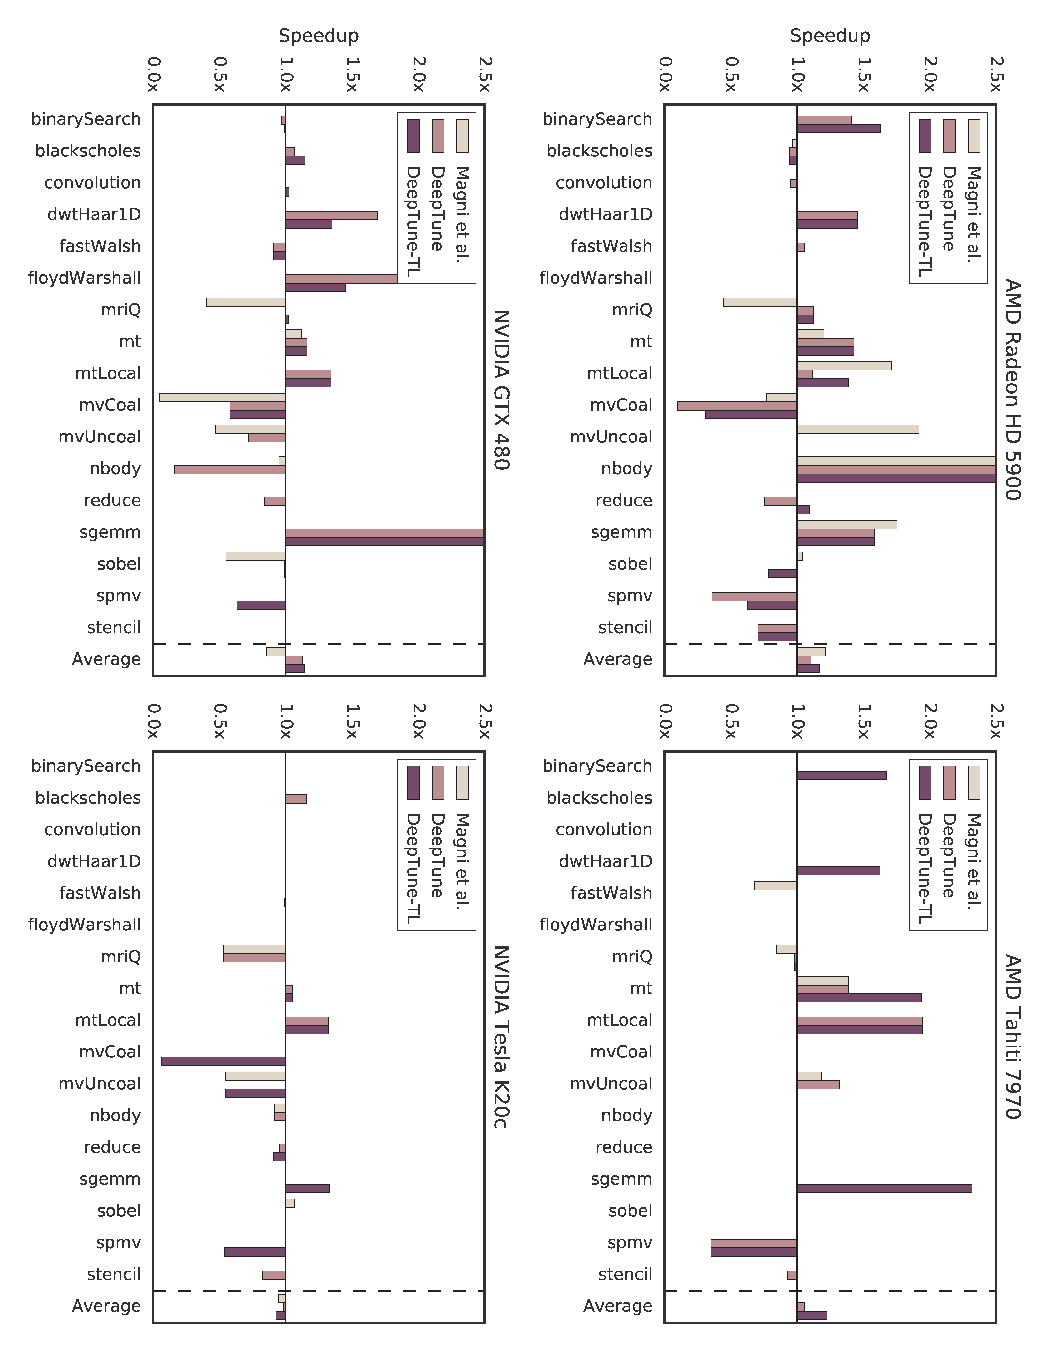
\includegraphics[width=\textwidth]{img/pact-speedup}%
	\caption[Speedups of predicted thread coarsening factors]{%
		Speedups of predicted coarsening factors for each platform. DeepTune outperforms \emph{Magni et al.\ }on three of the four platforms. Transfer learning improves DeepTune speedups further, by 16\% on average.%
	}%
	\label{fig:pact-speedup}
\end{figure}

On the NVIDIA Tesla K20c, the platform for which no predictive model achieves positive average speedups, DeepTune-TL matches or improve performance in the majority of cases, but over-coarsening on three of the programs causes a modest reduction in average performance. For this platform, further performance results are suspected necessary due to its unusual optimisation profile.


\section{DeepTune Internal Activation States}
\label{subsec:deeptune-internal-states}

In previous sections DeepTune is shown to automatically outperform state-of-the-art predictive models for which experts have invested a great amount of time in engineering features. This section attempts to illuminate the inner workings, using a single example from Case Study B: predicting the thread coarsening factor for Parboil's \texttt{mriQ} benchmark on four different platforms.

Figure~\ref{fig:viz} shows the DeepTune configuration, with visual overlays showing the internal state. From top to bottom, the input to the model is the 267 lines of OpenCL code for the \texttt{mriQ} kernel. This source code is preprocessed, formatted, and rewritten using variable and function renaming, shown in Figure~\ref{fig:viz}b. The rewritten source code is tokenised and encoded in a $1$-of-$k$ vocabulary. Figure~\ref{fig:viz}c shows the first 80 elements of this encoded sequence as a heat map in which each cell's colour reflects its encoded value. The input, rewriting, and encoding is the same for each of the four platforms.

\begin{figure*}
  \centering %
  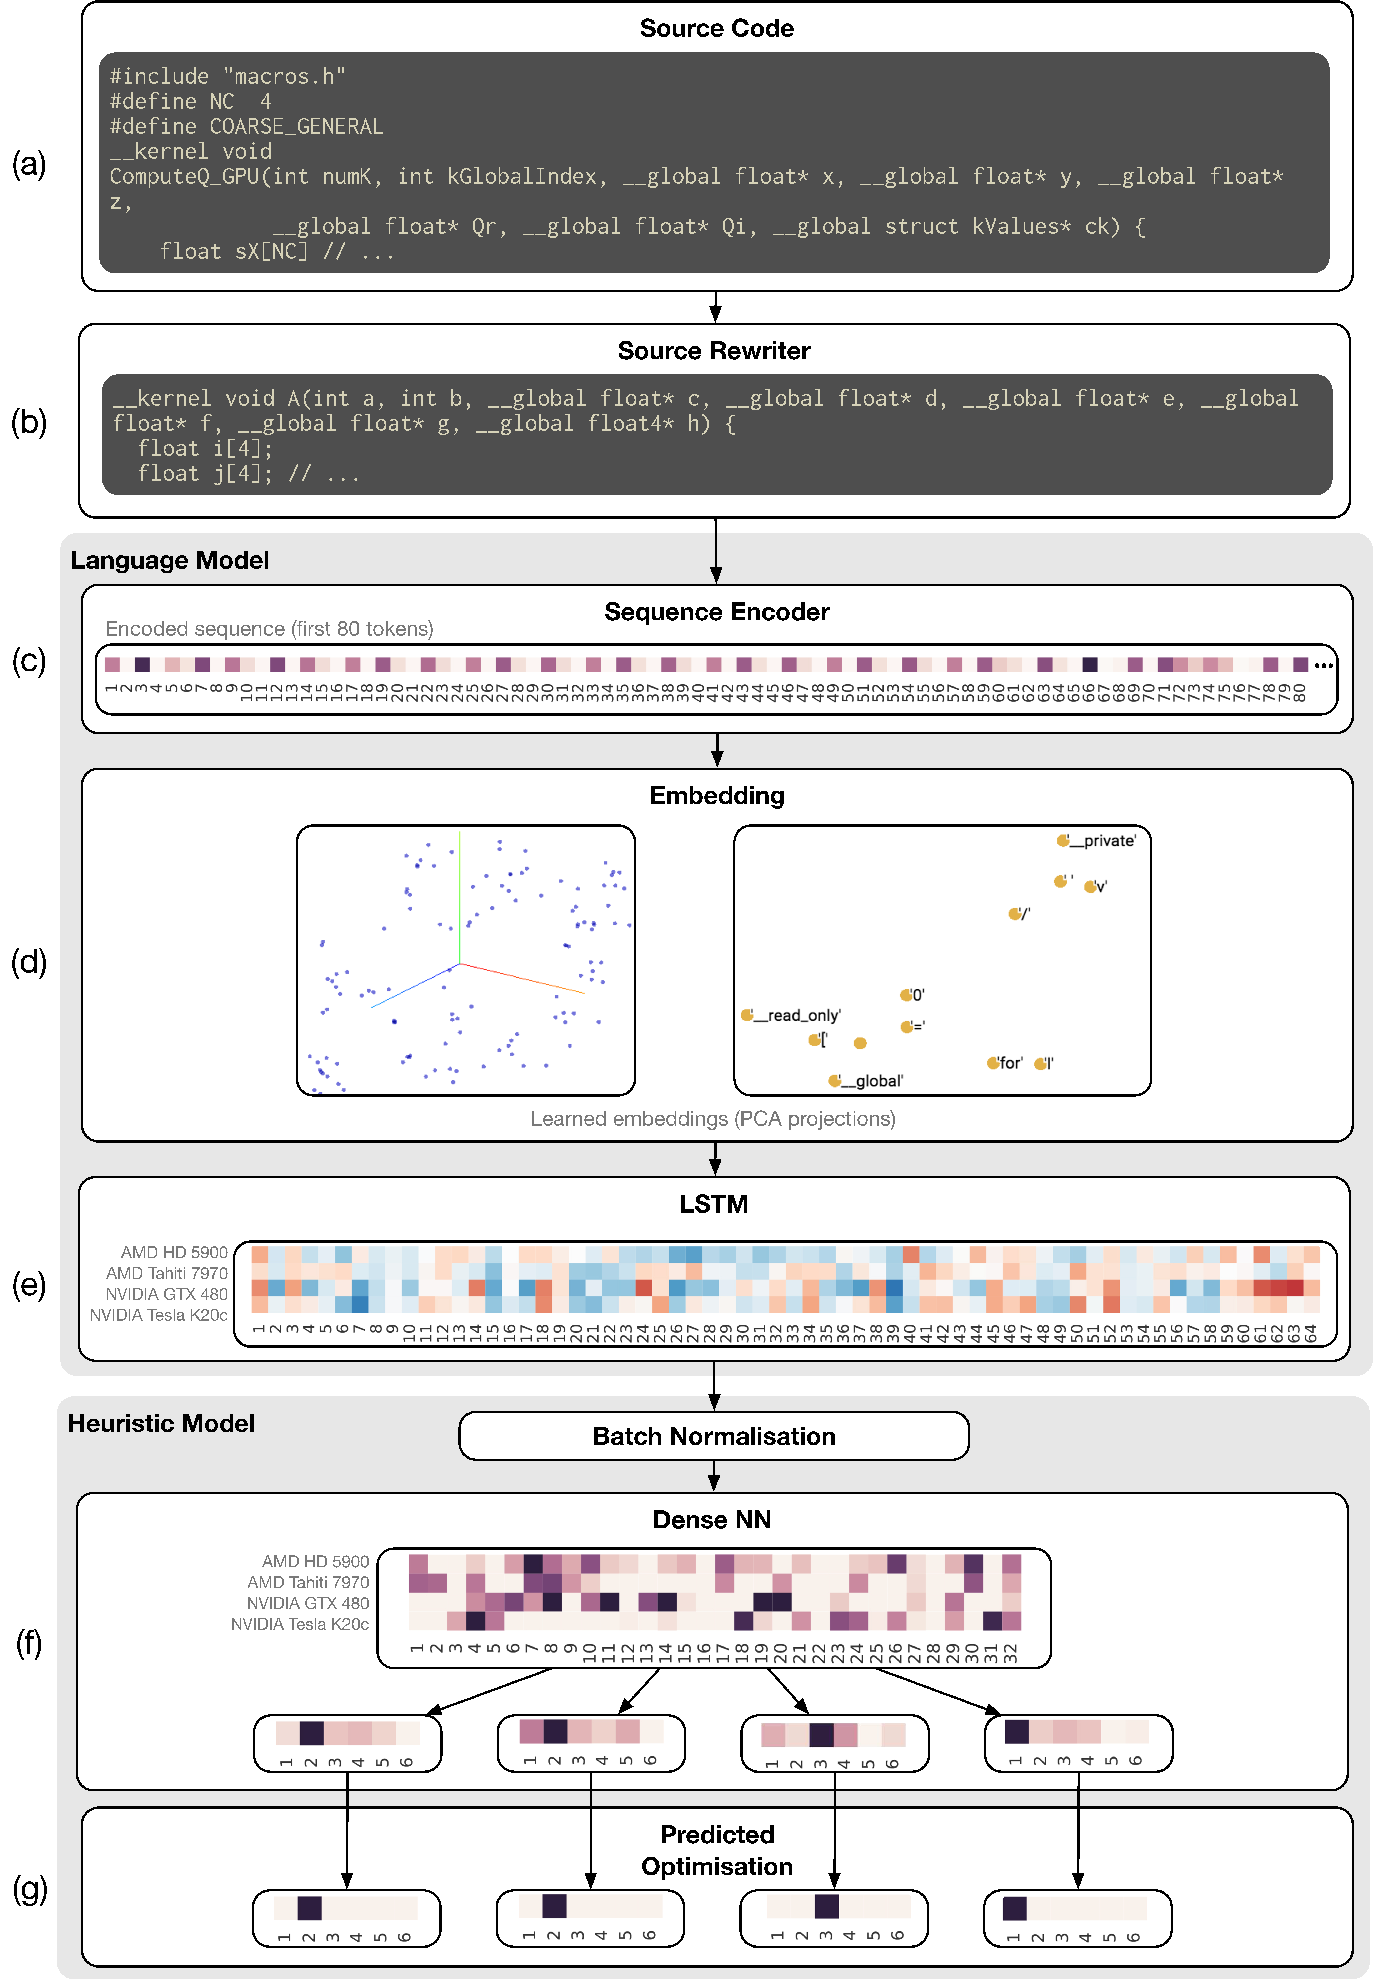
\includegraphics[width=\textwidth]{img/viz}%
    \vspace{-1em}
  \caption{%
    Visualizing the internal state of DeepTune when predicting coarsening factor
    for Parboil's \texttt{mriQ} benchmark on four different architectures. The
    activations in each layer of the four models increasingly diverge the lower
    down the network.%
  }
  \label{fig:viz} %
\end{figure*}


The encoded sequences are then passed into the Embedding layer. This maps each token of the vocabulary to a point in a 64 dimension vector space. Embeddings are learned during training so as to cluster semantically related tokens together. As such, they may differ between the four platforms. Figure~\ref{fig:viz}d shows a PCA projection of the embedding space for one of the platforms, showing multiple clusters of tokens. By honing in on one of the clusters and annotating each point with its corresponding token, it can be observed that the cluster contains the semantically related OpenCL address space modifiers \texttt{\_\_private}, \texttt{\_\_global}, and \texttt{\_\_read\_only}.

Two layers of 64 LSTM neurons model the sequence of embeddings, with the neuron activations of the second layer being used to characterise the entire sequence. Figure~\ref{fig:viz}e shows the neurons in this layer for each of the four platforms, using a red-blue heat map to visualise the intensity of each activation. Comparing the activations between the four platforms, we note a number of neurons in the layer with different responses across platforms. This indicates that the language model is partly specialised to the target platform. Subsequent experiments in~\cite{Ben-nun2018} support this reasoning, where a platform-agnostic language model achieves slightly poorer performance.

As information flows through the network, the layers become progressively more specialised to the specific platform. This can be seen in Figure~\ref{fig:viz}f, which shows the two layers of the heuristic model. The activations within these increasingly diverge. The mean variance of activations across platforms increases threefold compared to the language model, from 0.039 to 0.107. Even the activations of the AMD HD 5900 and AMD Tahiti 7970 platforms are dissimilar, despite the final predicted coarsening factor for both platforms being the same. The largest activation of the output layer is taken in Figure~\ref{fig:viz}g as the final predicted coarsening factor. For this particular program, a state-of-the-art model achieves 54\% of the maximum performance. DeepTune achieves 99\%.



%
%
%
%
%
%\section{Experimental Methodology}
%\label{sec:deeptune-methodology}
%
%DeepTune is applied to two heterogeneous compiler-based machine learning tasks and its performance compared to state-of-the-art approaches that use expert selected features.
%
%
%\subsection{Case Study A: OpenCL Heterogeneous Mapping}
%
%OpenCL provides a platform-agnostic framework for heterogeneous parallelism. This allows a program written in OpenCL to execute transparently across a range of different devices, from CPUs to GPUs and FPGAs. Given a program and a choice of execution devices, the question then is on which device should we execute the program to maximise performance?
%
%\subsubsection{State-of-the-art}
%
%In~\cite{Grewe2013}, \emph{Grewe et al.\ }develop a predictive model for mapping OpenCL kernels to the optimal device in CPU/GPU heterogeneous systems. They use supervised learning to construct decision trees, using a combination of static and dynamic kernel features. The static program features are extracted using a custom LLVM pass; the dynamic features are taken from the OpenCL runtime.
%
%\subsubsection{Expert Chosen Features}
%
%Table~\ref{tab:grewe-features-final} shows the features used by their work. Each feature is an expression built upon the code and runtime metrics given in Table~\ref{tab:grewe-features-raw}.
%
%\begin{table}
  \rowcolors{2}{gray!25}{white}
  \centering%
  \subfloat[Feature values]{
    \begin{tabular}{| l L{4.5cm} |}
      \hline
      \rowcolor{gray!50}
      \textbf{Name} & \textbf{Description} \\
      \hline
      \texttt{F1: data size/(comp+mem)} & commun.-computation ratio \\
      \texttt{F2: coalesced/mem} & \% coalesced memory accesses \\
      \texttt{F3: (localmem/mem)$\times$wgsize} & ratio local to global mem accesses  $\times$ \#.\ work-items \\
      \texttt{F4: comp/mem} & computation-mem ratio\\
      \hline
    \end{tabular}%
    \label{tab:grewe-features-final}%
  }\\ %
  \subfloat[Values used in feature computation]{%
    \rowcolors{2}{gray!25}{white}
    \begin{tabular}{| l c l |}
    	\hline
      \rowcolor{gray!50}
      \textbf{Name} & \textbf{Type} & \textbf{Description} \\
      \hline
      \texttt{comp} & static & \#.\ compute operations \\
      \texttt{mem} & static & \#.\ accesses to global memory \\
      \texttt{localmem} & static & \#.\ accesses to local memory \\
      \texttt{coalesced} & static & \#.\ coalesced memory accesses \\
      \texttt{data size} & dynamic & size of data transfers \\
      \texttt{work-group size} & dynamic & \#.\ work-items per kernel \\
      \hline
    \end{tabular}%
    \label{tab:grewe-features-raw}%
  }
  \caption[Heterogeneous mapping model features]{%
    Features used by \emph{Grewe et al. }to predict heterogeneous device
    mappings for OpenCL kernels.%
  } %
  \label{tab:grewe-features} %
\end{table}

%
%\subsubsection{Experimental Setup}
%
%The predictive model of \emph{Grewe et al.\ }~\cite{Grewe2013} is replicated. The same experimental setup is used as in Section~\ref{sec:clgen-eval-methodology} in which the experiments are extended to a larger set of 71 programs, summarised in Table~\ref{tab:cgo-benchmarks}. The programs were evaluated on two CPU-GPU platforms, detailed in Table~\ref{tab:cgo-platforms}.
%
%\begin{table}
\centering%
\rowcolors{2}{white}{gray!25}
\subfloat[Case Study A: OpenCL Heterogeneous Mapping]{%
  \begin{tabular}{l r r r}
    \toprule
    & \textbf{Version} & \textbf{\#. benchmarks} & \textbf{\#. kernels}\\
    \midrule
    \textbf{NPB (SNU~\cite{Seo2011})} & 1.0.3 & 7 & 114 \\
    \textbf{Rodinia~\cite{Che2009}} & 3.1 & 14 & 31 \\
    \textbf{NVIDIA SDK} & 4.2 & 6 & 12 \\
    \textbf{AMD SDK} & 3.0 & 12 & 16 \\
    \textbf{Parboil~\cite{Stratton2012}} & 0.2 & 6 & 8 \\
    \textbf{PolyBench~\cite{Grauer-Gray2012}} & 1.0 & 14 & 27 \\
    \textbf{SHOC~\cite{Danalis2010}} & 1.1.5 & 12 & 48 \\
    \textbf{Total} & - & 71 & 256 \\
    \bottomrule
  \end{tabular}
  \label{tab:cgo-benchmarks}
}\\*
\subfloat[Case Study B: OpenCL Thread Coarsening Factor]{%
  \begin{tabular}{l r r r}
    \toprule
    & \textbf{Version} & \textbf{\#. benchmarks} & \textbf{\#. kernels}\\
    \midrule
    \textbf{NVIDIA SDK} & 4.2 & 3 & 3 \\
    \textbf{AMD SDK} & 3.0 & 10 & 10 \\
    \textbf{Parboil~\cite{Stratton2012}} & 0.2 & 4 & 4 \\
    \textbf{Total} & - & 17 & 17 \\
    \bottomrule
  \end{tabular}
  \label{tab:pact-benchmarks}
}\\*
\caption{Benchmark programs.} %
\label{tab:benchmarks} %
\end{table}

%\begin{table}[t!]
  \centering %
  \subfloat[Case Study A: OpenCL Heterogeneous Mapping]{%
  \rowcolors{2}{gray!25}{white}
  \begin{tabular}{| l l l l| }
    \hline
    \rowcolor{gray!50}
    & \textbf{Frequency} & \textbf{Memory} & \textbf{Driver} \\
    \hline
    \textbf{Intel Core i7-3820} & 3.6 GHz & 8GB & AMD 1526.3 \\
    \textbf{AMD Tahiti 7970} & 1000 MHz & 3GB & AMD 1526.3 \\
    \textbf{NVIDIA GTX 970} & 1050 MHz & 4GB & NVIDIA 361.42 \\
    \hline
  \end{tabular}
  \label{tab:cgo-platforms}
  }\\*
  \subfloat[Case Study B: OpenCL Thread Coarsening Factor]{%
  \rowcolors{2}{gray!25}{white}
  \begin{tabular}{| l l l l |}
    \hline
    \rowcolor{gray!50}
    & \textbf{Frequency} & \textbf{Memory} & \textbf{Driver} \\
    \hline
    \textbf{AMD HD 5900} & 725 MHz & 2GB & AMD 1124.2 \\
    \textbf{AMD Tahiti 7970} & 1000 MHz & 3GB & AMD 1084.4 \\
    \textbf{NVIDIA GTX 480} & 700 MHz & 1536 MB & NVIDIA 304.54 \\
    \textbf{NVIDIA K20c} & 706 MHz & 5GB & NVIDIA 331.20 \\
    \hline
  \end{tabular}
  \label{tab:pact-platforms}
  }
  \caption{Experimental platforms.}
  \label{tab:platforms}
\end{table}

%
%\subsubsection{DeepTune Configuration} 
%
%Figure~\ref{fig:nn}a shows the neural network configuration of DeepTune for the task of predicting optimal device mapping. The OpenCL kernel source code is used as input, along with the two dynamic values \emph{work-group size} and \emph{data size} available to the OpenCL runtime.
%
%\subsubsection{Model Evaluation} 
%
%\emph{Stratified 10-fold cross-validation} is used to evaluate the quality of the predictive models~\cite{Han2011}. Each program is randomly allocated into one of 10 equally-sized sets; the sets are balanced to maintain a distribution of instances from each class consistent with the full set. A model is trained on the programs from all but one of the sets, then tested on the programs of the unseen set. This process is repeated for each of the 10 sets, to construct a complete prediction over the whole data set.
%
%\begin{figure}[t!]
  \centering
  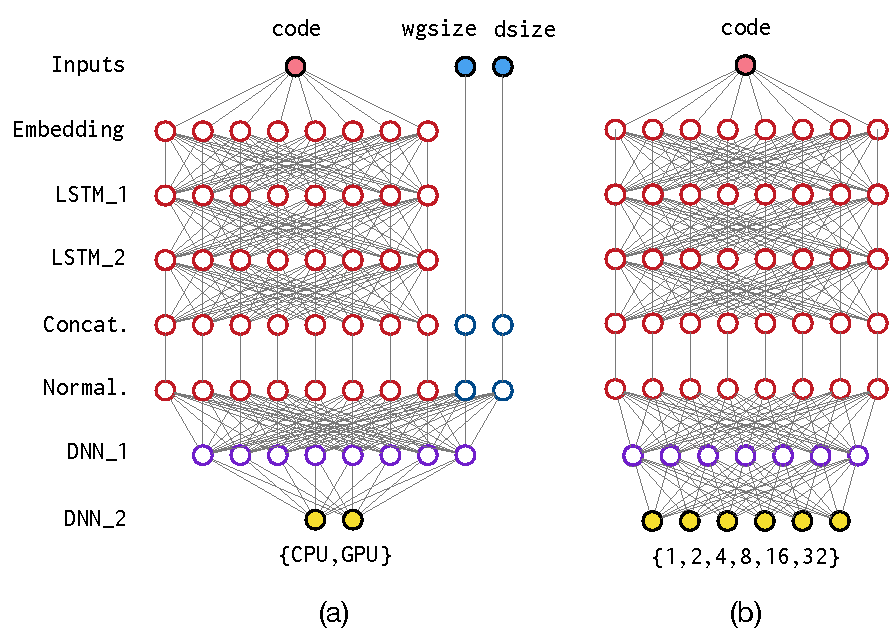
\includegraphics[width=\columnwidth]{img/nn} %
  \caption[DeepTune artificial neural networks]{%
    DeepTune artificial neural networks, configured for (a) heterogeneous mapping, and (b) thread coarsening factor. The design stays almost the same regardless of the optimisation problem. The only changes are the extra input for (a) and size of the output layers.%
  }%
  \label{fig:nn}
\end{figure}

%
%
%\subsection{Case Study B: OpenCL Thread Coarsening Factor}
%
%Thread coarsening is an optimisation for parallel programs in which the operations of two or more threads are fused together. This optimisation can prove beneficial on certain combinations of programs and architectures, for example programs with a large potential for Instruction Level Parallelism on Very Long Instruction Word architectures.
%
%\subsubsection{State-of-the-art} \emph{Magni et al.\ }present a predictive model for OpenCL thread coarsening in~\cite{Magni2014}. They implement an iterative heuristic which determines whether a given program would benefit from coarsening. If yes, then the program is coarsened, and the process repeats, allowing further coarsening. In this manner, the problem is reduced from a multi-label classification problem into a series of binary decisions, shown in Figure~\ref{fig:cf-magni}. They select from one of six possible coarsening factors: $(1, 2, 4, 8, 16, 32)$, divided into 5 binary choices.
%
%\begin{figure}
  \centering %
  \subfloat[Magni \emph{et al.\ }cascading binary model.]{%
    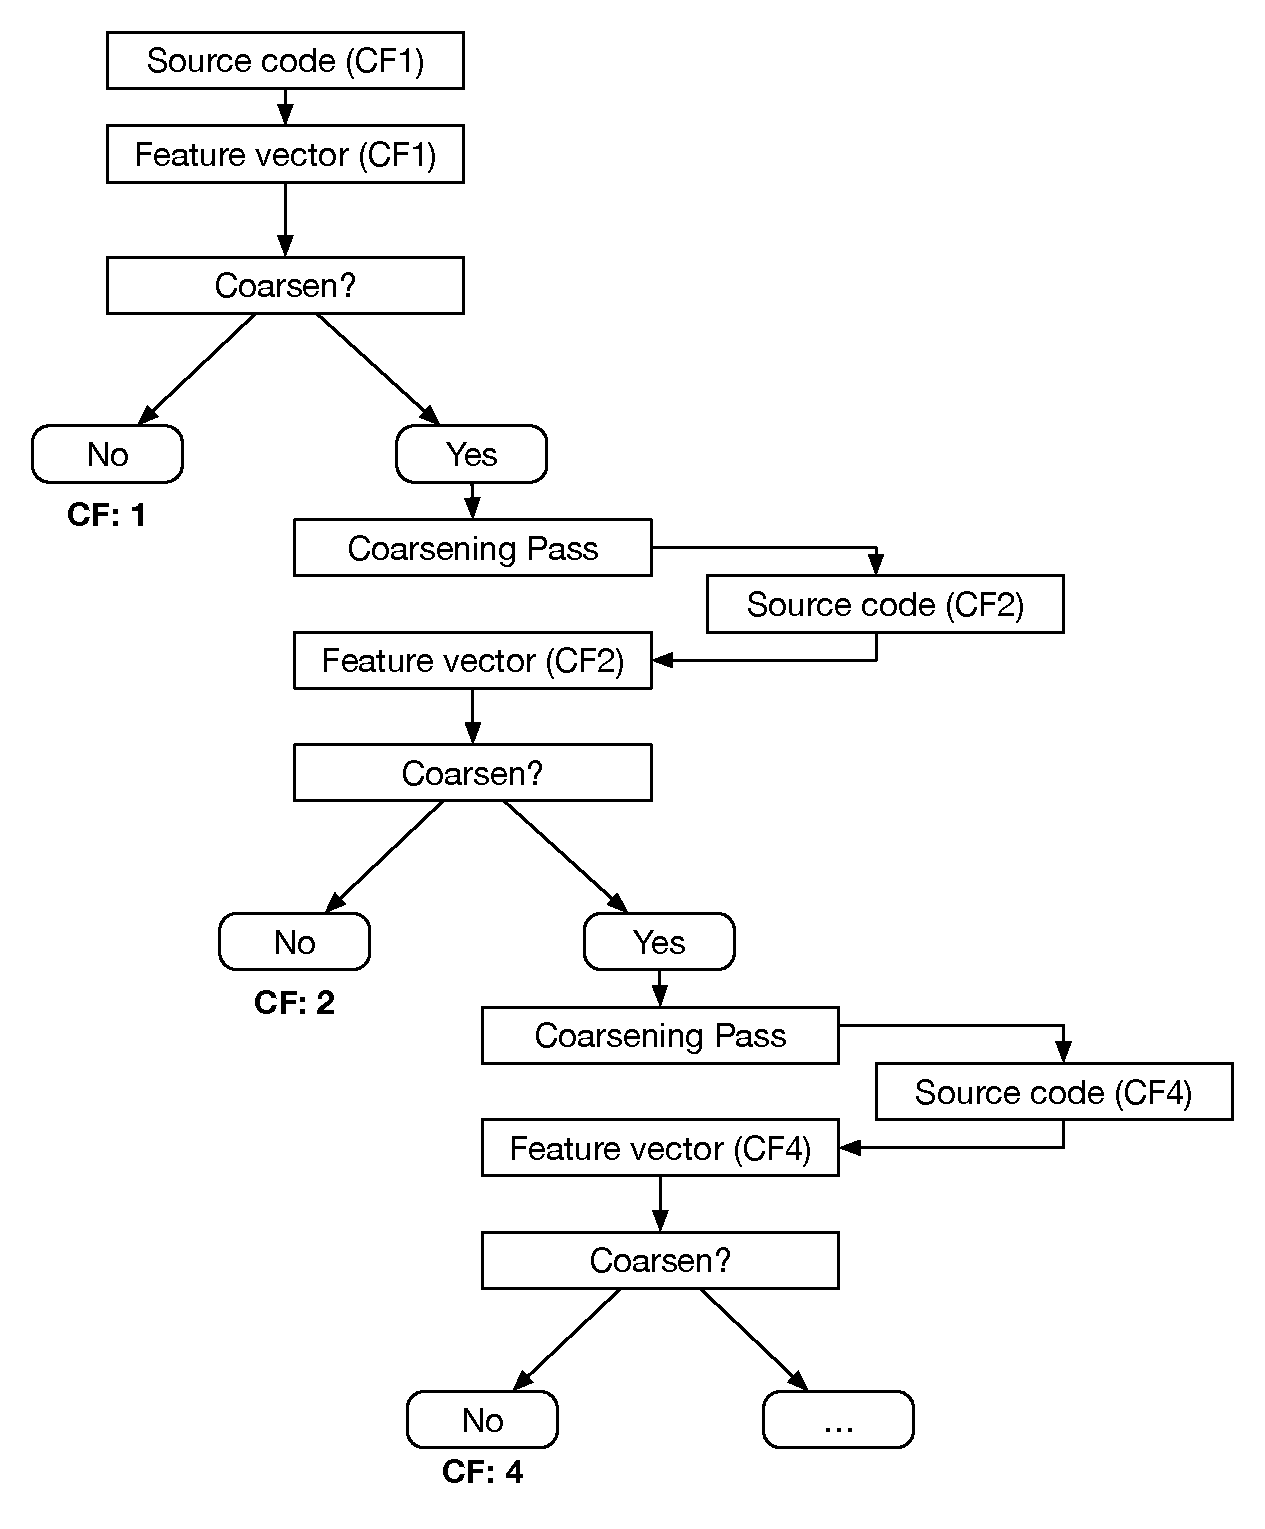
\includegraphics[width=.85\columnwidth]{img/cf-magni}%
    \label{fig:cf-magni}
  }\\*%
  \subfloat[Our approach.]{%
      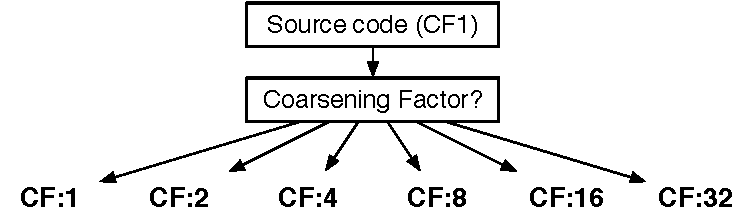
\includegraphics[width=.65\columnwidth]{img/cf-deeptune}%
      \label{fig:cf-deeptune}
  }%
  \caption{%
      Two approaches for predicting coarsening factor (CF) of OpenCL kernels.
      Magni \emph{et al.\ }reduce the multi-label classification problem to a
      series of binary decisions, by iteratively applying the optimization and
      computing new feature vectors. Our approach simply predicts the coarsening
      factor directly from the source code.%
  }
  \label{fig:cascading-nn}
\end{figure}

%
%\begin{table}
  \rowcolors{2}{gray!25}{white}
  \centering%
    \begin{tabular}{| l l |}
      \hline
      \rowcolor{gray!50}
      \textbf{Name} & \textbf{Description} \\
      \hline
      \texttt{BasicBlocks} & \#.\ basic blocks \\
      \texttt{Branches} & \#.\ branches \\
      \texttt{DivInsts} & \#.\ divergent instructions \\
      \texttt{DivRegionInsts} & \#.\ instructions in divergent regions \\
      \texttt{DivRegionInstsRatio} & \#.\ instr. in divergent regions / total instructions \\
      \texttt{DivRegions} & \#.\ divergent regions \\
      \texttt{TotInsts} & \#.\ instructions \\
      \texttt{FPInsts} & \#.\ floating point instructions \\
      \texttt{ILP} & average ILP / basic block \\
      \texttt{Int/FP Inst Ratio} & \#.\ branches \\
      \texttt{IntInsts} & \#.\ integer instructions \\
      \texttt{MathFunctions} & \#.\ match builtin functions \\
      \texttt{MLP} & average MLP / basic block \\
      \texttt{Loads} & \#.\ loads \\
      \texttt{Stores} & \#.\ stores \\
      \texttt{UniformLoads} & \#.\ loads unaffected by coarsening direction \\
      \texttt{Barriers} & \#.\ barriers \\
      \hline
    \end{tabular}%
    \label{tab:features-pact14-raw}%
  \caption[\emph{Magni et al.\ }features for predicting thread coarsening]{%
    Candidate features used by \emph{Magni et al.\ }for predicting thread
    coarsening. From these values, they compute relative deltas for each
    iteration of coarsening, then use PCA for selection.%
  }%
  \label{tab:magni-features} %
\end{table}

%
%\subsubsection{Expert Chosen Features}
%
%\emph{Magni et al.\ }followed a very comprehensive feature engineering process. 17 candidate features were assembled from previous studies of performance counters and computed theoretical values~\cite{Magni2,Sim2012}. For each candidate feature they compute its coarsening \emph{delta}, reflecting the change in each feature value caused by coarsening: $f_{\Delta} = (f_{after} - f_{before}) / f_{before}$, adding it to the feature set. Then they use Principle Component Analysis (PCA) on the 34 candidates and selected the first 7 principle components, accounting for 95\% of variance in the space.
%
%\subsubsection{Experimental Setup}
%
%The experimental setup of \emph{Magni et al.}~\cite{Magni2014} is replicated. The thread coarsening optimisation is evaluated on 17 programs, listed in Table~\ref{tab:pact-benchmarks}. Four different GPU architectures are used, listed in Table~\ref{tab:pact-platforms}.
%
%\subsubsection{DeepTune Configuration}
%
%Figure~\ref{fig:nn}b shows the neural network configuration. The OpenCL kernel is the sole input the coarsening factor is the predicted output.
%
%\subsubsection{Model Evaluation}
%
%Compared to Case Study A, the size of the evaluation is small. We use \emph{leave-one-out cross-validation} to evaluate the models. For each program, a model is trained on data from all other programs and used to predict the coarsening factor of the excluded program.
%
%The parameters of the neural network is not described in~\cite{Magni2014}, so an additional, \emph{nested} cross-validation process is used to find the optimal model parameters. For every program in the training set, 48 combinations of network parameters are evaluated. The best performing configuration is selected from these 768 results to train a model for prediction on the excluded program. This nested cross-validation is repeated for each of the training sets. No such tuning of hyper-parameters is performed for DeepTune.
%
%
%\subsection{Comparison of Case Studies}
%
%For the two different optimisation heuristics, the authors arrived at very different predictive model designs, with very different features. By contrast, the DeepSmith approach is exactly the same for both problems. None of DeepTune's parameters were tuned for the case studies presented above. Their settings represent conservative choices expected to work reasonably well for most scenarios.
%
%Table~\ref{tab:nn-size} shows the similarity of the models. The only difference between the network designs is the auxiliary inputs for Case Study A and the different number of optimisation decisions. The differences between DeepTune configurations is only two lines of code: the first, adding the two auxiliary inputs; the second, increasing the size of the output layer for Case Study B from two neurons to six. The description of these differences is larger than the differences themselves.
%
%\begin{table}
  \centering
  \rowcolors{2}{white}{gray!25}
  \begin{tabular}{| l r r | r r |}
    \hline
    \rowcolor{gray!50}
    & \multicolumn{2}{c}{\textbf{\#.\ neurons}} & \multicolumn{2}{c}{\textbf{\#.\ parameters}} \\
    \rowcolor{gray!50}
    & \textbf{HM} & \textbf{CF} & \textbf{HM} & \textbf{CF} \\
    \hline
    \textbf{Embedding} & 64 & 64 & ,256 & 8,256 \\
    \textbf{LSTM\_1} & 64 & 64 & 33,024 & 33,024 \\
    \textbf{LSTM\_2} & 64 & 64 & 33,024 & 33,024 \\
    \textbf{Concatenate} & 64 + 2 & - & - & - \\
    \textbf{Batch Normalisation} & 66 & 64 & 264 & 256 \\
    \textbf{DNN\_1} & 32 & 32 & 2,144 & 2,080 \\
    \textbf{DNN\_2} & 2 & 6 & 66 & 198 \\
    \hline
    \textbf{Total} & & & 76,778 & 76,838 \\
    \hline
  \end{tabular}
  \caption[DeepTune model parameters]{%
    The size and number of parameters of the DeepTune components of
    Figure~\ref{fig:nn}, configured for heterogeneous mapping (HM) and
    coarsening factor (CF).%
  }
  \label{tab:nn-size}
\end{table}


\section{Qualitative Evaluation of Generated Programs}\label{sec:eval}

In this section we evaluate the quality of programs synthesized by CLgen by their likeness to hand-written code.

% \subsection{Likeness to Hand-written Code}

Judging whether a piece of code has been written by a human is a challenging task for a machine, so we adopt a methodology from machine learning research based on the \emph{Turing Test}~\cite{Gao2015a,Zhang2016,Vinyals}. We reason that if the output of CLgen is human like code, then a human judge will be unable to distinguish it from hand-written code.

We devised a double blind test in which 15 volunteer OpenCL developers from industry and academia were shown 10 OpenCL kernels each. Participants were tasked with judging whether, for each kernel, they believed it to have been written by hand or by machine. Kernels were randomly selected for each participant from two equal sized pools of synthetically generated and hand-written code from GitHub. We applied the code rewriting process to all kernels to remove comments and ensure uniform identifier naming. The participants were divided into two groups, with 10 of them receiving code generated by CLgen, and 5 of them acting as a control group, receiving code generated by CLSmith~\cite{Lidbury2015a}, a program generator for differential testing\footnote{An online version of this test is available at \emph{http://humanorrobot.uk/}.}.

We scored each participant's answers, finding the average score of the control group to be 96\% (stdev.\ 9\%), an unsurprising outcome as generated programs for testing have multiple ``tells'', for example, their only input is a single \texttt{ulong} pointer. There were no false positives (synthetic code labeled human) for CLSmith, only false negatives (human code labeled synthetic). With CLgen synthesized programs, the average score was 52\% (stdev.\ 17\%), and the ratio of errors was even. This suggests that CLgen code is indistinguishable from hand-written programs, with human judges scoring no better than random chance.

\section{Related Work}\label{sec:rw}

% \cc{TODO: ASPLOS reviewer suggestions~\cite{Yan2017}.}

% \cc{TODO: interesting recent work on Ocaml~\cite{Midtgaard2017}, jsfunfuzz, AFL, libFuzzer.}

The random generation of test cases is a well established approach to the compiler validation problem. Prior approaches are surveyed in~\cite{Kossatchev2005,Boujarwah1997} and empirically contrasted in~\cite{Chen2014a}. The main question of interest is in how to efficiently generate codes which trigger bugs. There are two main approaches: \emph{program generation}, in which inputs are synthesized from scratch, typically by stochastic enumeration of a grammar; and \emph{program mutation}, in which existing codes are modified and mutated so as to identify anomalous behavior.

\begin{figure}
	\centering %
	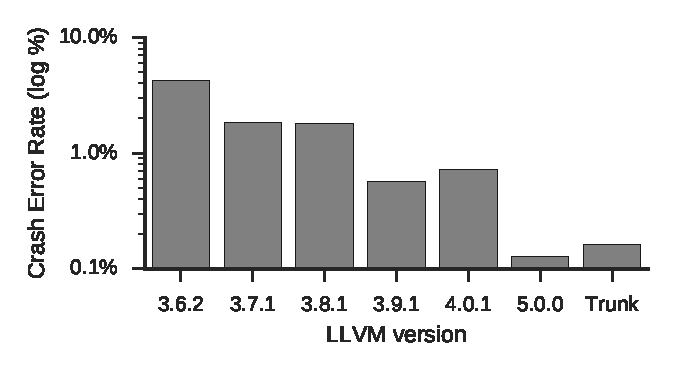
\includegraphics[width=.85\columnwidth]{build/img/clang-crashes}%
	\caption{%
		Crash rate of the Clang front-end of every LLVM release in the past 24 months compiling 75k DeepSmith kernels.
	}%
  \vspace{-0.8em}
	\label{fig:clangs} %
\end{figure}
\begin{table}
	\footnotesize %
	\centering %
	\begin{tabular}{r|ccccccc}
\toprule
{} & 3.6.2 & 3.7.1 & 3.8.1 & 3.9.1 & 4.0.1 & 5.0.0 & Trunk \\
\midrule
Assertion 1 &  2962 &  1327 &  1332 &   414 &   523 &    83 &    97 \\
Assertion 2 &       &     1 &     1 &       &       &       &       \\
Assertion 3 &       &       &       &       &       &       &     1 \\
Assertion 4 &       &       &       &       &       &       &     2 \\
Assertion 5 &   147 &       &       &       &       &       &       \\
Assertion 6 &     1 &       &       &       &       &       &       \\
Assertion 7 &       &       &       &     1 &     1 &       &       \\
Unreachable &    86 &    42 &    14 &    14 &    18 &    13 &    21 \\
\bottomrule
\end{tabular}

	\caption{%
		The number of DeepSmith programs which trigger distinct Clang front-end assertions, and the number of programs which trigger unreachables.%
	}
  \vspace{-3.1em}
	\label{tab:clangs}
\end{table}

\paragraph{Program Generation}

In the foundational work on differential testing for compilers, McKeeman \emph{et al.\ }present generators capable of enumerating programs of a range of qualities, from random ASCII sequences to C model conforming programs~\cite{McKeeman1998}. Subsequent works have presented increasingly complex generators which improve on the prior in some metric of interest, generally expressiveness or probability of correctness. CSmith~\cite{Yang2011} is a widely known and effective generator which enumerates programs by pairing infrequently combined language features. In doing so, it produces correct programs with clearly defined behavior but very unlikely functionality, increasing the chances of triggering a bug. Achieving this required extensive engineering work, most of it not portable across languages, and ignoring some language features. Subsequent generators influenced by CSmith, like Orange3~\cite{Nagai2013}, focus on features and bug types beyond the scope of CSmith, arithmetic bugs in the case of Orange3.

\paragraph{Program Mutation}

Equivalence Modulo Inputs (EMI) testing~\cite{Le2013a,Sun2016a} follows a different approach to test case generation. Starting with existing code, it inserts or deletes statements that will not be executed, so functionality should remain the same. If it is affected, it is due to a compiler bug. While a powerful technique able to find hard to detect bugs, it relies on having a very large number of programs to mutate. As such, it still requires an external code generator. Similarly to CSmith, EMI favors very long test programs. LangFuzz~\cite{Holler2012} also uses mutation but does this by inserting code segments which have previously exposed bugs. This increases the chances of discovering vulnerabilities in scripting language engines.
% \cc{TODO: Expand discussion}
Skeletal program enumeration~\cite{Zhang2017a} again works by transforming existing code. It identifies algorithmic patterns in short pieces of code and enumerates all the possible permutations of variable usage.
% \cc{TODO: no testing of invalid inputs, unclear if scales to complex programs.}

\paragraph{Test case Reduction} With both generation and mutation based approaches, bug-exposing programs can be unnecessarily long. While 80\% of the test cases related to GCC and LLVM bugs are 45 lines~\cite{Sun2016} or less, CSmith/EMI output tends to be thousands of lines long. Most this code is not related to the bug and has to be removed for compiler engineers to understand the source of the problem. To that end test case reduction techniques~\cite{Regehr2012a,Pflanzer2016,Herfert} have been developed to bring the code down to manageable lengths. These techniques are very slow, potentially taking several hours to reduce a single test case. Automated reducers also require extensive engineering effort, applying analyses at every stage of the iterative reduction process so as not to obscure the bug-exposing property of interest. Another common problem is prioritizing the most important bugs out of the hundreds or thousands discovered. This \emph{fuzz taming problem} is addressed in~\cite{Chen2013}, in which a distance metric is used to rank test cases such that diverse, interesting test cases are highly ranked. % \cc{TODO: Our approach complements EMI}

Compared to all these, our fuzzing approach is low cost, easy to develop, portable, capable of detecting a wide range of errors, and focusing by design on bugs that are more likely to be encountered in a production scenario.


%CSmith~\cite{Yang2011} and CLSmith~\cite{Lidbury2015a}. Same testing methodology, but very different design goals to our work. The explore the space of \emph{unlikely} programs, by pairing infrequently combined language features. Because Csmith programs are free form undefined behavior, there is only a single interpretation. This allows oracle-less differential testing across compilers, using a voting heuristic to identify erroneous compiler outputs. The ``shape'' of programs generated by Csmith is expert driven. The shape of programs generated by DeepSmith is data driven. The 80 probabilities which control Csmith program generation are extensively hand tuned to produce programs which ``look right''. Our data driven approach does not require this. In fact, our approach is portable across changing usage of a programming language.

%The functionality of Csmith is also expert driven. Every language feature supported by Csmith must be laboriously hand crafted, and results in a very complex system of over 40,000 lines of C++ code (which still omits many language features used in real programs, like heap allocation). The language features supported by DeepSmith is bound only by those which have been used on GitHub. DeepSmith has a non-zero probability of generating programs using every language feature found on GitHub. We reason that if a language feature remains unused in the entirety of code on GitHub, then it is reasonable to assume that it is not a feature worth testing. Both Csmith and CLsmith use unrealistic safe-math macros to wrap arithmetic operations. We do not.


% Increasing complexity of generations: RandProg to CSmith. Then EMI testing, and SPE.

%The \emph{fuzz taming problem} is addressed in~\cite{Chen2013}, in which a distance metric is used to rank test cases such that diverse, interesting test cases are highly ranked.

%\emph{LangFuzz} attempts a similar approach of learning to generate test cases from real code~\cite{Holler2012}. For LangFuzz, the input programs are codes known to have previously exposed bugs.

%Empirical comparison of compiler testing techniques~\cite{Chen2014a}

%\cc{is it wise to draw attention to this?} If the output of a program depends on undefined or unspecified behavior, then comparing outputs across compilers is meaningless. Prior works have formulated random program generation so as to minimize or eradicate the possibility of undefined and unspecified behavior~\cite{Yang2011c,Le2013a,Le2015}, at the expense of expressiveness. Recently, work in Skeletal Program Enumeration~\cite{Zhang2017a} has relied on handchecking of C programs and tools such as CompCert~\cite{Leroy2013} and UBsan to detect false-positives. Since DeepSmith programs are not guaranteed to be free from undefined behaviors, and we can only determine if a program is well-formed empirically, additional filtering of test cases is required to prevent false-positives.

%Analysis of bugs in GCC and LLVM finds 80\% of test cases to be 45 lines~\cite{Sun2016}.

%\cc{TODO}~\cite{Godefroid2008a,Le2015,Sun2016a}~\cite{Kossatchev2005}.

%\cc{TODO:} Directed EMI testing~\cite{Le2015}.

%\cc{TODO: finding arithmetic bugs which CSmith cannot~\cite{Nagai2013}}

%``As a matter of implementation quality, a compiler vendor will usually fix a segmentation fault or similar problem even if the crash-inducing test case, for example, uses a variable without initialization.''~\cite{Regehr2012a}

%Skeletal program enumeration~\cite{Zhang2016a}. By enumerating entire program space, provides bounded guarantees of compiler correctness. Same shortcoming as CSmith (well formed programs only). No OpenCL implementation. Probably would take a lot of development effort. \cc{More investigation required.}

%Both tools require test case reduction (\cite{Regehr2012a} and~\cite{Pflanzer2016}, respectively). Work in test case reduction~\cite{Regehr2012a} reduced Csmith program sizes by 74--594$\times$ while preserving the bug exposing behavior. They median reduced CSmith program size they found was only 20 lines (0.5KB).

%\cc{TODO:}

%EMI testing~\cite{Le2013a}, Skeletal Program enumeration~\cite{Zhang2017a}.

%Fuzzing with code fragments~\cite{Holler2012}.

%A mutation-based approach for the Java Virtual Machine is demonstrated in~\cite{Chena}.

%TODO~\cite{White2016},~\cite{Sheridan2007}.

%Grammar-base whitebox testing~\cite{Godefroid2008a}.

%Our unique contribution is a low cost method for fuzzing, capable of detecting a wide range of errors, and matching that of human expectation (small, plausible test cases).


%HJL - Removing - \paragraph{GPU Testing} \pp{Do we really need this?} GPU Concurrency --- Small \emph{litmus tests}~\cite{Alglave2015}.
%GPUVerify~\cite{Bardsley2014}.

\paragraph{Machine Learning} In software testing,
machine learning has been successfully applied before on areas such as improving bug finding static analyzers~\cite{Heo2017,Koc2017}, repairing programs~\cite{Koukoutos2017a,White}, prioritizing test programs~\cite{Chen2017}, identifying buffer overruns~\cite{Choi2016}, and processing bug reports~\cite{Lam2016,Huo2016}. A proof-of-concept implementation of machine learning for input fuzzing is presented in~\cite{Godefroid2017}, although no bugs are found. % TODO: More on this?

\begin{table}
	\footnotesize %
	\centering %
	\begin{tabular}{rc|ccc}
\toprule
  \textbf{Compiler} & $\pm$ & \textbf{Silent Crashes} & \textbf{Assertion 1} & \textbf{Assertion 2}\\
\midrule
  \multirow{ 2}{*}{solc} & $-$ & 204 & 1 & \\
                         & $+$ & 204 & 1 & \\
  \hline
  \multirow{ 2}{*}{solc-js} & $-$ & 3628 & 1 & 1\\
                         & $+$ & 908 & 1 & 1\\
\bottomrule
\end{tabular}
	\caption{%
		% Results from 12 hours of testing Solidity compilers using DeepSmith.
		The number of DeepSmith programs that trigger Solidity compiler crashes from 12 hours of testing.%
     \vspace{-1em}
	}
   \vspace{-2em}
	\label{tab:solidity}
\end{table}

% \cite{Yan2017}

Deep Learning is a nascent field that is responsible for a multitude of breakthroughs in modeling rich, hierarchical datasets. The major milestones are reviewed in~\cite{Wang2017}, and methods in~\cite{Schmidhuber2014}. There is an increasing interest in mining source code repositories at large scale~\cite{Allamanis2017a}.
% \cc{Using machine learning to inductive program synthesis~\cite{Parisotto2016,Balog2017}.}
Previous studies have involved data mining of GitHub to analyze software engineering practices~\cite{Wu2014,Guzman2014,Baishakhi2014a,Vasilescu2015}, for example code generation~\cite{Zhang2015a}, comment generation~\cite{Wong2013}, and code completion~\cite{Raychev2014}.
% \cc{Creating compilable code snippets mined from StackOverflow~\cite{Terragni2016}}.
To the best of our knowledge, no work so far has succeeded in finding compiler bugs by exploiting mined source code for test case generation. Ours is the first to do so.

\section{Summary}%
\label{sec:conclusion}

Applying machine learning to compiler and runtime optimizations requires generating features first. This is a time consuming process, it needs supervision by an expert, and even then we cannot be sure that the selected features are optimal. In this paper we present a novel tool for building optimization heuristics, DeepTune, which forgoes feature extraction entirely, relying on powerful language modeling techniques to automatically build effective representations of programs directly from raw source code. The result translates into a huge reduction in development effort, improved heuristic performance, and more simple model designs.

Our approach is fully automated. Using DeepTune, developers no longer need to spend months using statistical methods and profile counters to select program features via trial and error. It is worth mentioning that we do not tailor our model design or parameters for the optimization task at hand, yet we achieve performance on par with and in most cases \emph{exceeding} state-of-the-art predictive models.

We used DeepTune to automatically construct heuristics for two challenging compiler and runtime optimization problems, find that, in both cases, we outperform state-of-the-art predictive models by 14\% and 12\%. We have also shown that the DeepTune architecture allows us to exploit information learned from another optimization problem to give the learning a boost. Doing so provides up to a 16\% performance improvement when training using a handful of programs. We suspect this approach will be useful in other domains for which training data are a scarce resource.

In future work, we will extend our heuristic construction approach by automatically learning dynamic features over raw data; apply unsupervised learning techniques~\cite{Le2012} over unlabeled source code to further improve learned representations of programs; and deploy trained DeepTune heuristic models to low power embedded systems using quantization and compression of neural networks~\cite{Han2015}.


\bibliographystyle{unsrt}
\bibliography{refs}


\end{document}
\endinput
